\subsection{Client}
Racchiude tutte le componenti necessarie per il front-end del prodotto. Visualizza i dati dell'utente e invia richieste al server.
\begin{figure}[H]
\centering
\noindent\makebox[\textwidth]{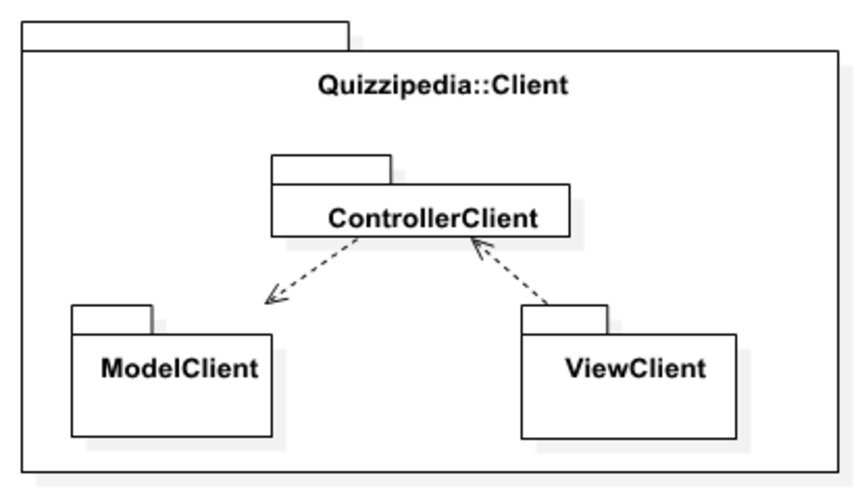
\includegraphics[width=\textwidth]{ImgST/quizzipedia-client.pdf}}
\caption{Schema Componente Quizzipedia::Client}
\end{figure}
\subsubsection{Componente Quizzipedia::Client::ModelClient}
Rappresenta il modello dei dati che verranno utilizzati dal sistema lato client.
\begin{figure}[H]
\centering
\noindent\makebox[\textwidth]{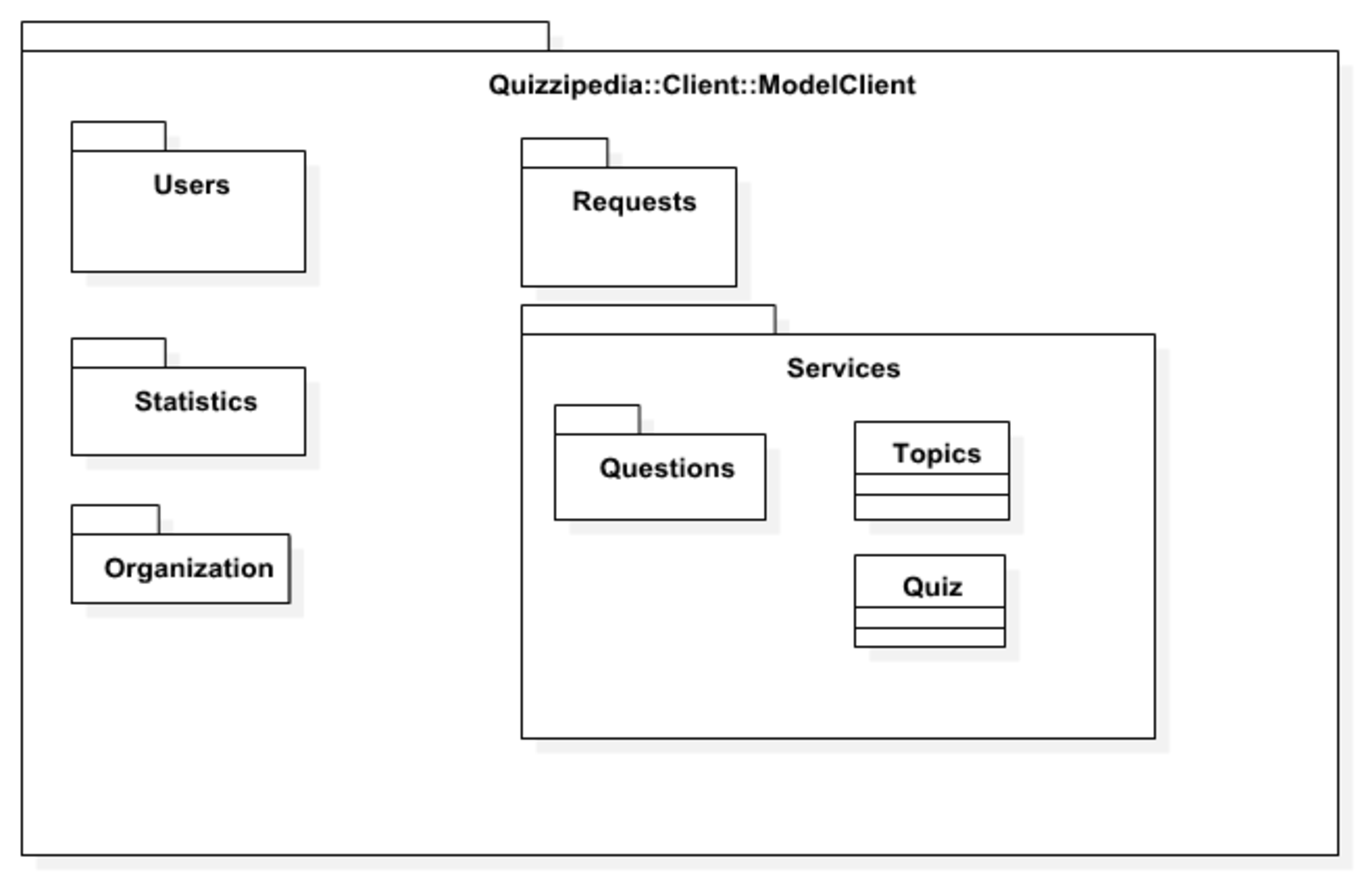
\includegraphics[width=\textwidth]{ImgST/quizzipedia-client-modelclient.pdf}}
\caption{Schema Componente Quizzipedia::Client::ModelClient}
\end{figure}
\myparagraph{Componenti contenute}
\begin{itemize}
\item Quizzipedia::Client::ModelClient::Organization
\item Quizzipedia::Client::ModelClient::Requests
\item Quizzipedia::Client::ModelClient::Services
\item Quizzipedia::Client::ModelClient::Statistics
\item Quizzipedia::Client::ModelClient::Users
\end{itemize}
\subsubsection{Componente Quizzipedia::Client::ModelClient::Organization}
La componente gestisce le classi e gli enti, ovvero il sistema in base a cui sono organizzati gli utenti nel sistema.
\begin{figure}[H]
\centering
\noindent\makebox[\textwidth]{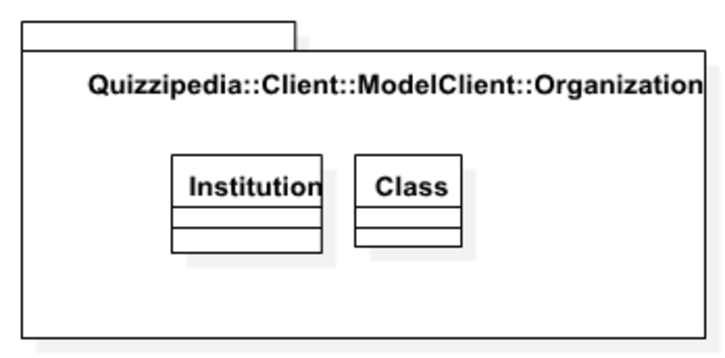
\includegraphics[width=\textwidth]{ImgST/quizzipedia-client-modelclient-organization.pdf}}
\caption{Schema Componente Quizzipedia::Client::ModelClient::Organization}
\end{figure}
\myparagraph{Classe Class}
Contiene informazioni relative alla struttura delle classi.
\begin{figure}[H]
\centering
\noindent\makebox[\textwidth]{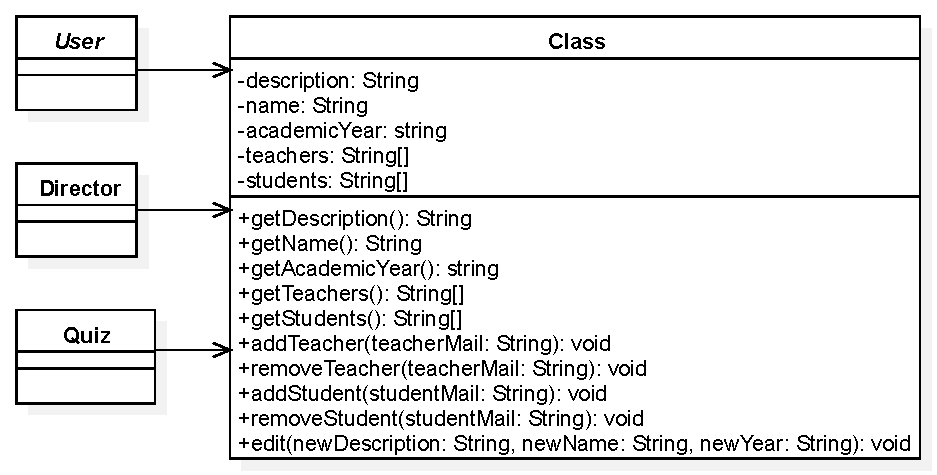
\includegraphics[width=\textwidth]{ImgST/quizzipedia-client-modelclient-organization-class.pdf}}
\caption{Schema Componente Quizzipedia::Client::ModelClient::Organization::Class}
\end{figure}
\mysubparagraph{Relazioni con altre classi}
\begin{itemize}
\item Quizzipedia::Client::ModelClient::Organization::Institution
\end{itemize}
\subsubsection{Componente Quizzipedia::Client::ModelClient::Requests}
Questo package contiene le classi necessarie a gestire le richieste di ruolo e di classe degli utenti.
\begin{figure}[H]
\centering
\noindent\makebox[\textwidth]{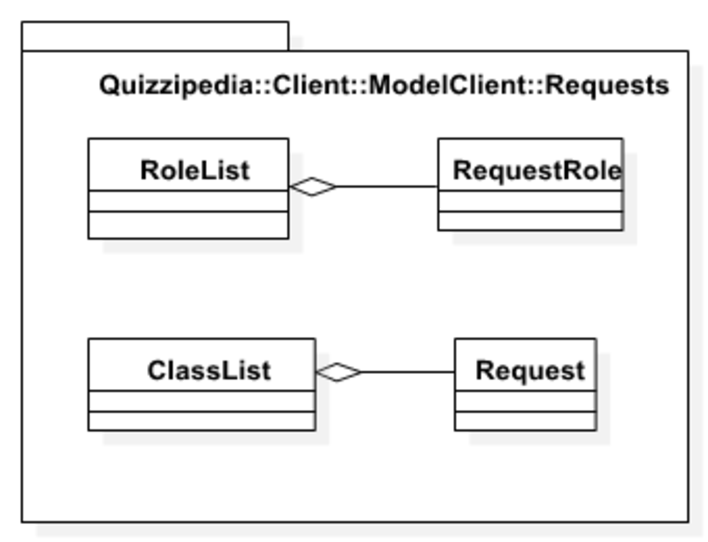
\includegraphics[width=\textwidth]{ImgST/quizzipedia-client-modelclient-requests.pdf}}
\caption{Schema Componente Quizzipedia::Client::ModelClient::Requests}
\end{figure}
\myparagraph{Classe ClassList}
Questa classe gestisce le richieste da parte di Docenti o Studenti per l'assegnazione a una specifica classe.
\begin{figure}[H]
\centering
\noindent\makebox[\textwidth]{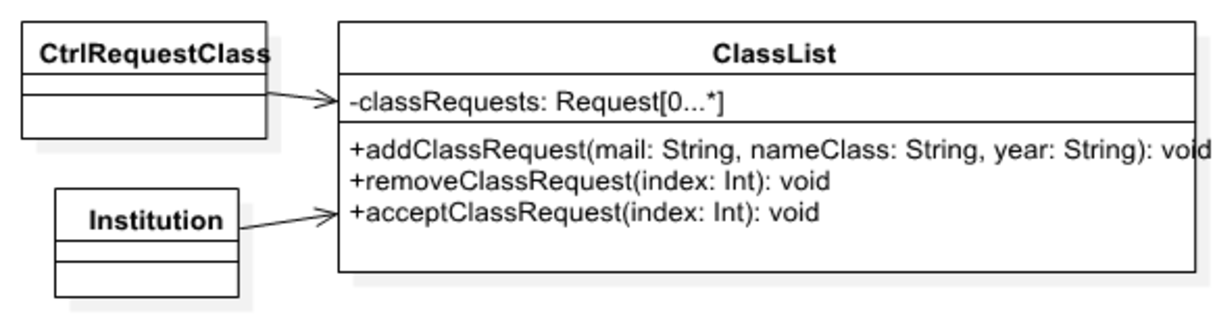
\includegraphics[width=\textwidth]{ImgST/quizzipedia-client-modelclient-requests-classlist.pdf}}
\caption{Schema Componente Quizzipedia::Client::ModelClient::Requests::ClassList}
\end{figure}
\mysubparagraph{Relazioni con altre classi}
\begin{itemize}
\item Quizzipedia::Client::ModelClient::Requests::Request
\end{itemize}
\subsubsection{Componente Quizzipedia::Client::ModelClient::Services}
Il package racchiude i modelli necessari alla creazione di domande e quiz, i servizi principali offerti dal nostro prodotto.
\begin{figure}[H]
\centering
\noindent\makebox[\textwidth]{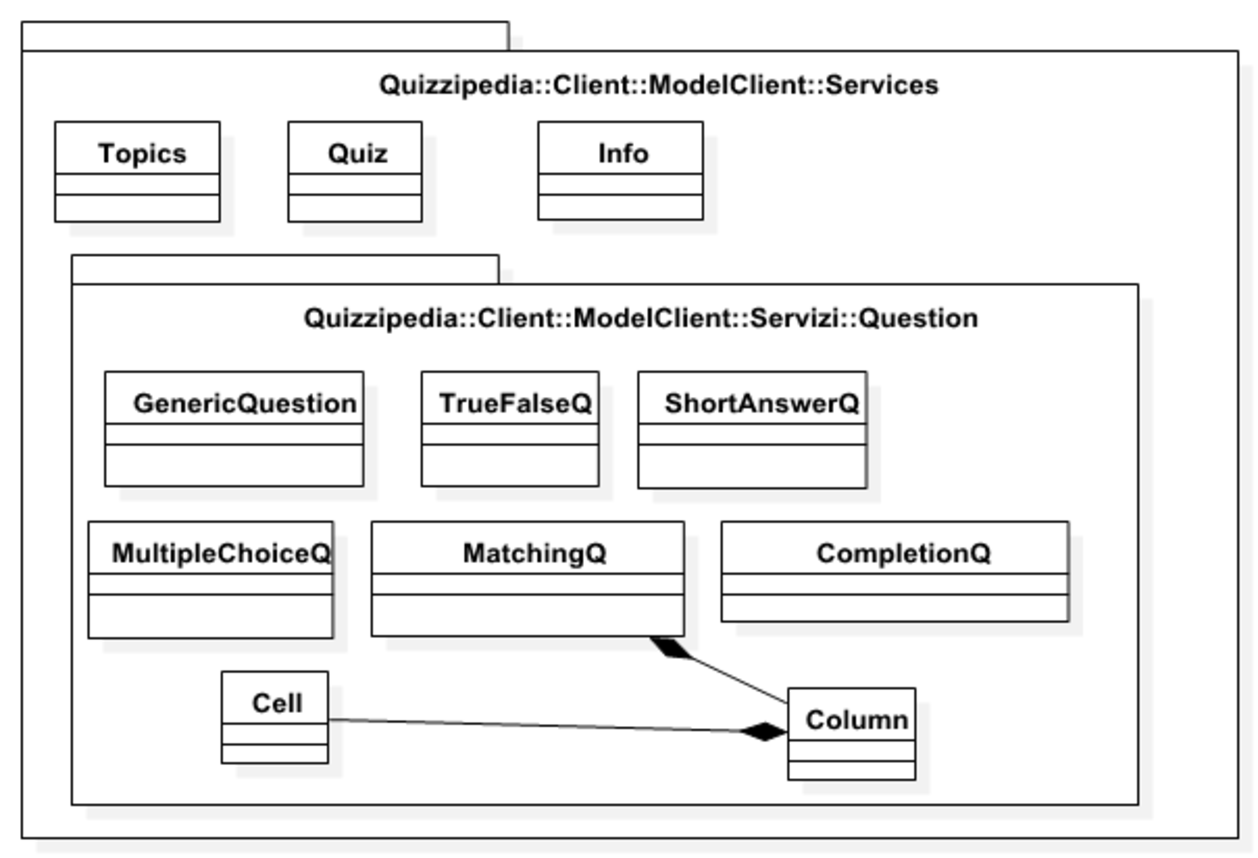
\includegraphics[width=\textwidth]{ImgST/quizzipedia-client-modelclient-services.pdf}}
\caption{Schema Componente Quizzipedia::Client::ModelClient::Services}
\end{figure}
\myparagraph{Componenti contenute}
\begin{itemize}
\item Quizzipedia::Client::ModelClient::Services::Questions
\end{itemize}
\myparagraph{Classe Info}
Riassume le informazioni principali su quiz e domande, necessarie per una presentazione sintetica e puntuale all'utente. È poi possibile risalire alla domanda o al quiz completi.
\begin{figure}[H]
\centering
\noindent\makebox[\textwidth]{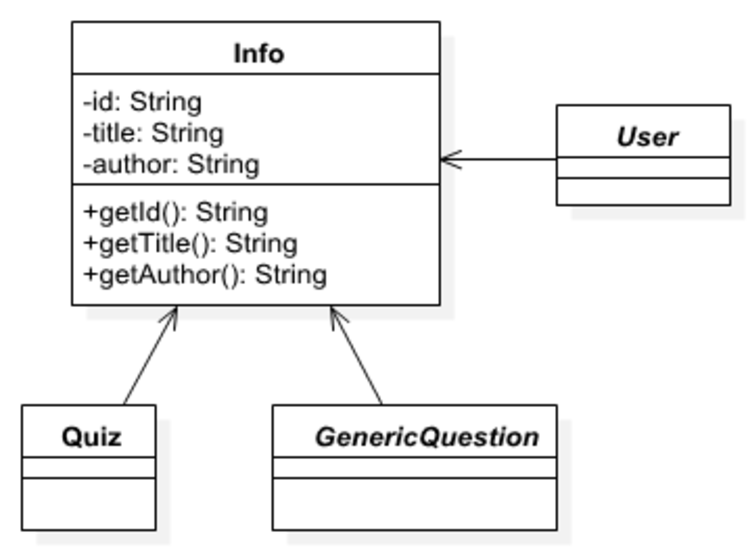
\includegraphics[width=\textwidth]{ImgST/quizzipedia-client-modelclient-services-info.pdf}}
\caption{Schema Componente Quizzipedia::Client::ModelClient::Services::Info}
\end{figure}
\subsubsection{Componente Quizzipedia::Client::ModelClient::Services::Questions}
Descrive il modo in cui sono strutturati i vari tipi di domande che l'utente può incontrare durante la creazione o la compilazione di quiz.
\begin{figure}[H]
\centering
\noindent\makebox[\textwidth]{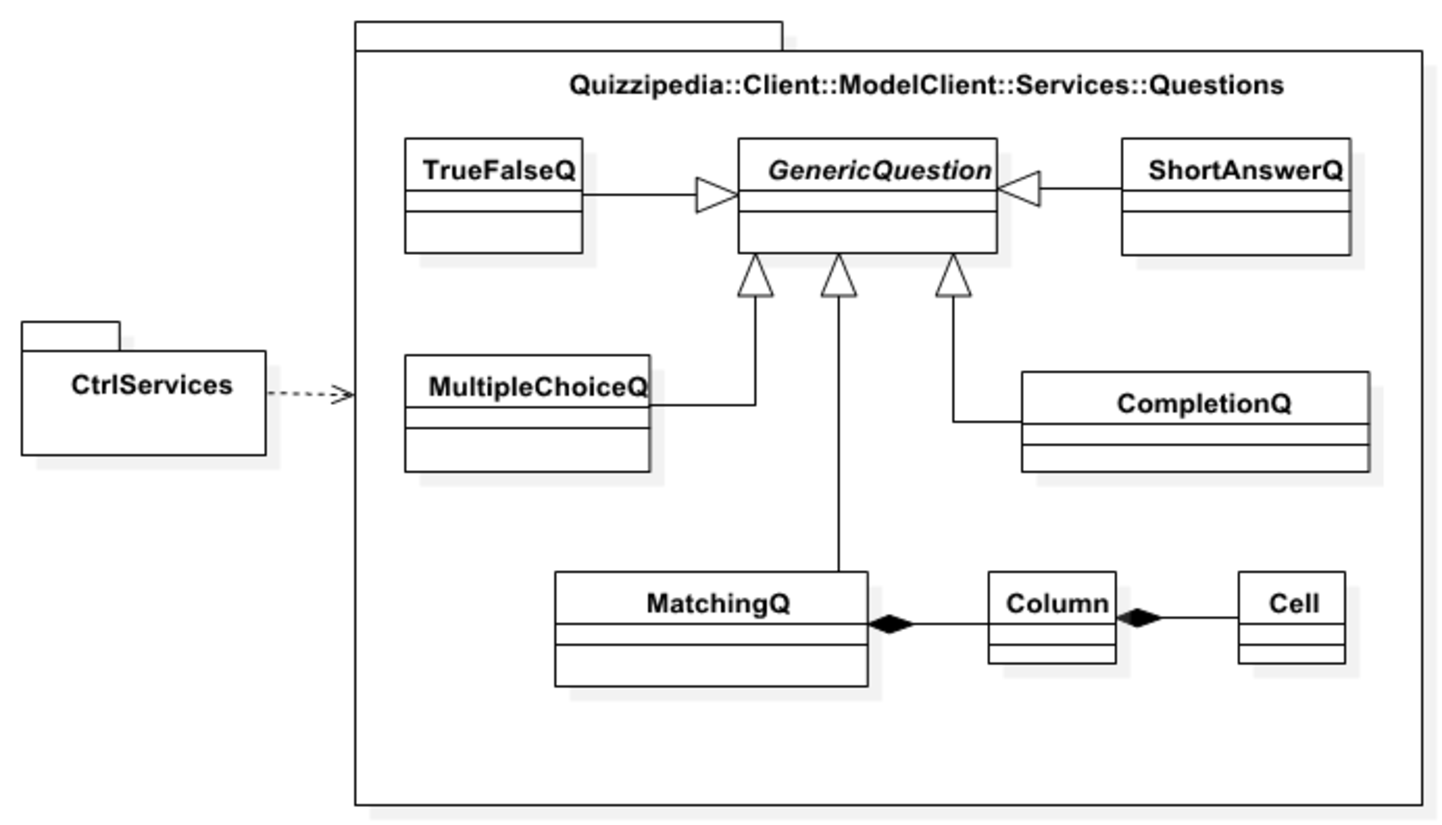
\includegraphics[width=\textwidth]{ImgST/quizzipedia-client-modelclient-services-questions.pdf}}
\caption{Schema Componente Quizzipedia::Client::ModelClient::Services::Questions}
\end{figure}
\myparagraph{Classe Cell}
La classe descrive ogni singola riga (quindi ogni opzione) della colonna della domanda a collegamento.
\begin{figure}[H]
\centering
\noindent\makebox[\textwidth]{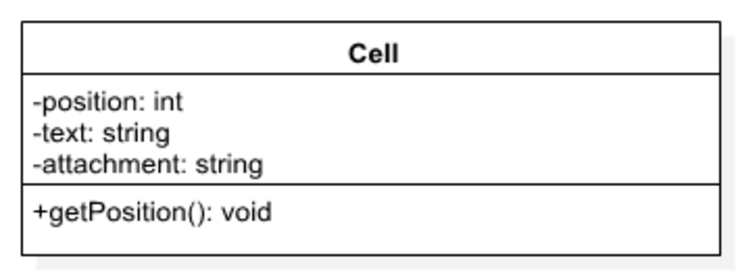
\includegraphics[width=\textwidth]{ImgST/quizzipedia-client-modelclient-services-questions-cell.pdf}}
\caption{Schema Componente Quizzipedia::Client::ModelClient::Services::Questions::Cell}
\end{figure}
\subsubsection{Componente Quizzipedia::Client::ModelClient::Statistics}
Qui sono raccolte le classi con il compito di reperire informazioni sulle statistiche dal server e presentarle al'utente finale. Sono disponibili statistiche per le domande, per i quiz e per gli studenti di ogni classe.
\begin{figure}[H]
\centering
\noindent\makebox[\textwidth]{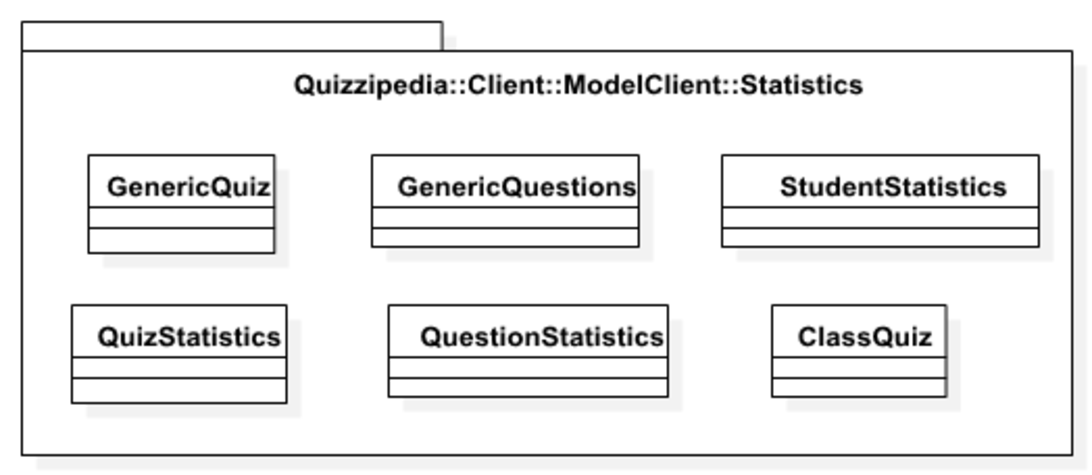
\includegraphics[width=\textwidth]{ImgST/quizzipedia-client-modelclient-statistics.pdf}}
\caption{Schema Componente Quizzipedia::Client::ModelClient::Statistics}
\end{figure}
\myparagraph{Classe ClassQuiz}
La classe raccoglie le statistiche riguardanti gli studenti di una classe relativamente a un quiz assegnato.
\begin{figure}[H]
\centering
\noindent\makebox[\textwidth]{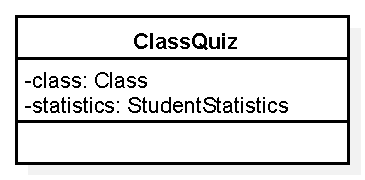
\includegraphics[width=\textwidth]{ImgST/quizzipedia-client-modelclient-statistics-classquiz.pdf}}
\caption{Schema Componente Quizzipedia::Client::ModelClient::Statistics::ClassQuiz}
\end{figure}
\mysubparagraph{Relazioni con altre classi}
\begin{itemize}
\item Quizzipedia::Client::ModelClient::Statistics::StudentStatistics
\end{itemize}
\subsubsection{Componente Quizzipedia::Client::ModelClient::Users}
Raccoglie le classi necessarie a descrivere le diverse tipologie di utente che possono accedere al sistema.
\begin{figure}[H]
\centering
\noindent\makebox[\textwidth]{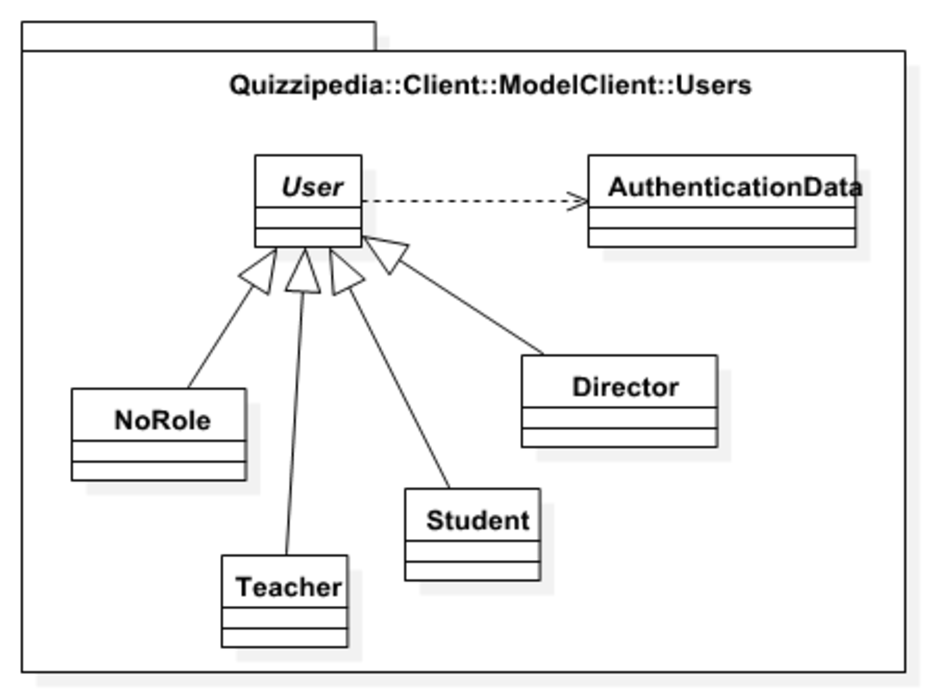
\includegraphics[width=\textwidth]{ImgST/quizzipedia-client-modelclient-users.pdf}}
\caption{Schema Componente Quizzipedia::Client::ModelClient::Users}
\end{figure}
\myparagraph{Classe AutheniticationData}
Questa classe gestisce le informazioni di autenticazione comuni a tutti gli utenti.
\begin{figure}[H]
\centering
\noindent\makebox[\textwidth]{\includegraphics[width=\textwidth]{ImgST/quizzipedia-client-modelclient-users-autheniticationdata.pdf}}
\caption{Schema Componente Quizzipedia::Client::ModelClient::Users::AutheniticationData}
\end{figure}
\mysubparagraph{Relazioni con altre classi}
\begin{itemize}
\item Quizzipedia::Client::ModelClient::Users::User
\end{itemize}
\subsubsection{Componente Quizzipedia::Client::ViewClient}
Racchiude tutte le componenti necessarie per presentare il prodotto all'utente.
\begin{figure}[H]
\centering
\noindent\makebox[\textwidth]{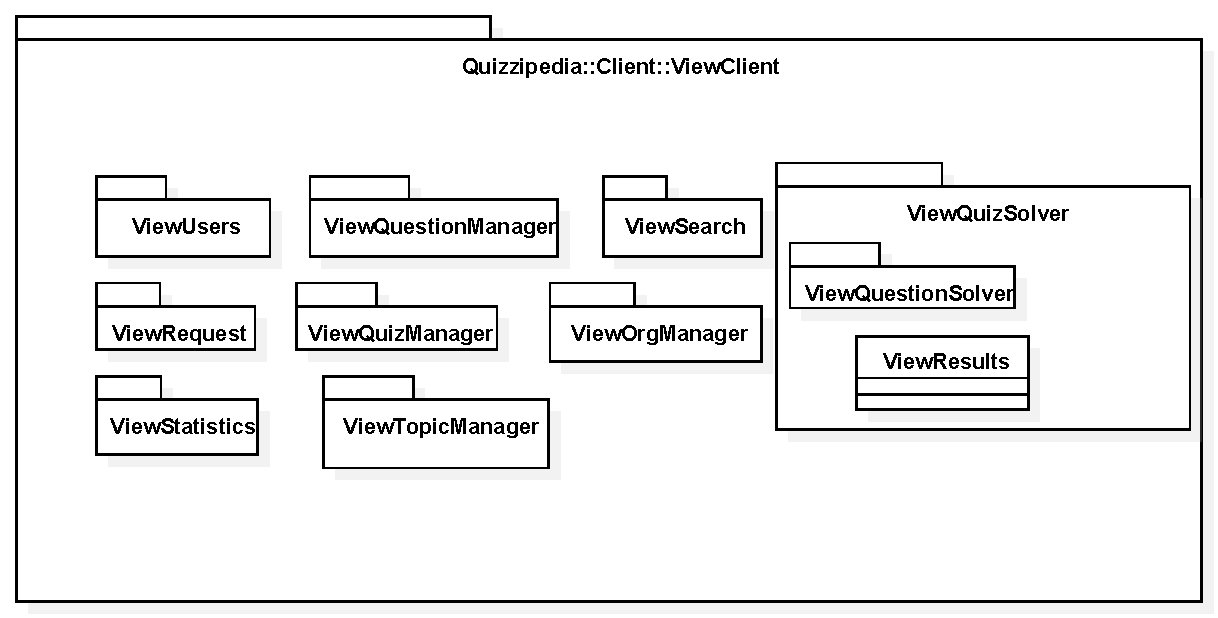
\includegraphics[width=\textwidth]{ImgST/quizzipedia-client-viewclient.pdf}}
\caption{Schema Componente Quizzipedia::Client::ViewClient}
\end{figure}
\myparagraph{Componenti contenute}
\begin{itemize}
\item Quizzipedia::Client::ViewClient::ViewClassManager
\item Quizzipedia::Client::ViewClient::ViewQuestionManager
\item Quizzipedia::Client::ViewClient::ViewQuizManager
\item Quizzipedia::Client::ViewClient::ViewQuizSolver
\item Quizzipedia::Client::ViewClient::ViewRequests
\item Quizzipedia::Client::ViewClient::ViewSearch
\item Quizzipedia::Client::ViewClient::ViewStatistics
\item Quizzipedia::Client::ViewClient::ViewTopicManager
\item Quizzipedia::Client::ViewClient::ViewUsers
\end{itemize}
\subsubsection{Componente Quizzipedia::Client::ViewClient::ViewClassManager}
Qui sono raccolte le classi responsabili della presentazione delle pagine da cui sarà possibile gestire le classi.
\begin{figure}[H]
\centering
\noindent\makebox[\textwidth]{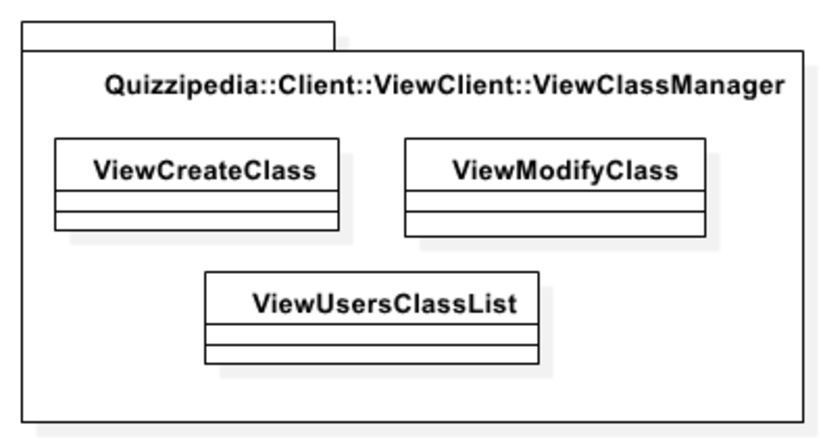
\includegraphics[width=\textwidth]{ImgST/quizzipedia-client-viewclient-viewclassmanager.pdf}}
\caption{Schema Componente Quizzipedia::Client::ViewClient::ViewClassManager}
\end{figure}
\myparagraph{Classe ViewCreateClass}
Classe responsabile di creare la pagina da cui sarà possibile creare una nuova classe.
\begin{figure}[H]
\centering
\noindent\makebox[\textwidth]{\includegraphics[width=\textwidth]{ImgST/quizzipedia-client-viewclient-viewclassmanager-viewcreateclass.pdf}}
\caption{Schema Componente Quizzipedia::Client::ViewClient::ViewClassManager::ViewCreateClass}
\end{figure}
\subsubsection{Componente Quizzipedia::Client::ViewClient::ViewQuestionManager}
Qui sono raccolte le classi responsabili della presentazione delle pagine da cui sarà possibile gestire le domande.
\begin{figure}[H]
\centering
\noindent\makebox[\textwidth]{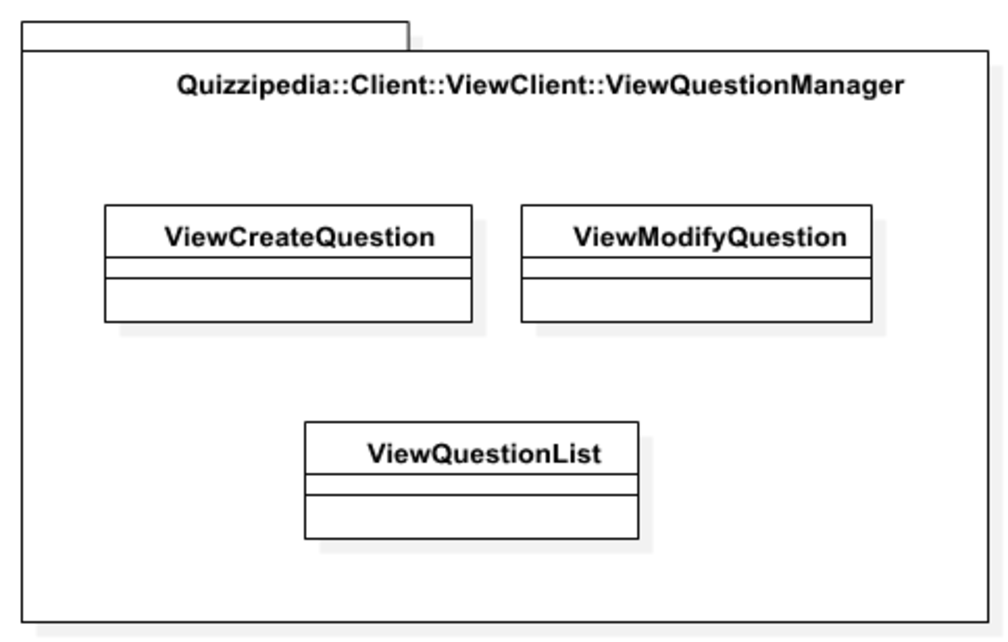
\includegraphics[width=\textwidth]{ImgST/quizzipedia-client-viewclient-viewquestionmanager.pdf}}
\caption{Schema Componente Quizzipedia::Client::ViewClient::ViewQuestionManager}
\end{figure}
\myparagraph{Classe ViewCreateQuestion}
Presenta la pagina da cui sarà possibile creare una nuova domanda.
\begin{figure}[H]
\centering
\noindent\makebox[\textwidth]{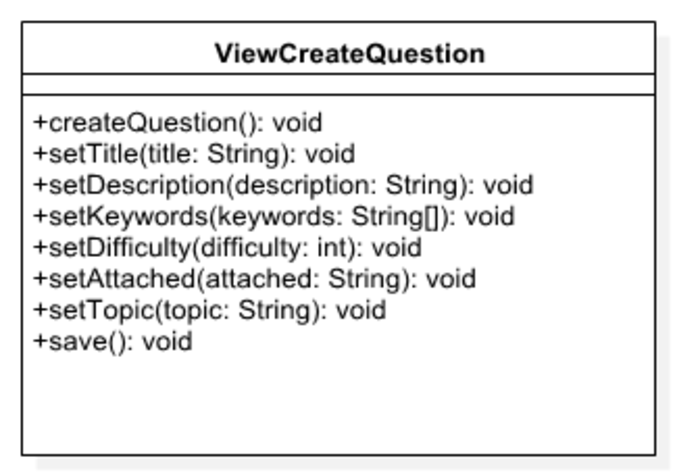
\includegraphics[width=\textwidth]{ImgST/quizzipedia-client-viewclient-viewquestionmanager-viewcreatequestion.pdf}}
\caption{Schema Componente Quizzipedia::Client::ViewClient::ViewQuestionManager::ViewCreateQuestion}
\end{figure}
\subsubsection{Componente Quizzipedia::Client::ViewClient::ViewQuizManager}
Qui sono raccolte le classi responsabili della presentazione delle pagine da cui sarà possibile gestire i quiz.
\begin{figure}[H]
\centering
\noindent\makebox[\textwidth]{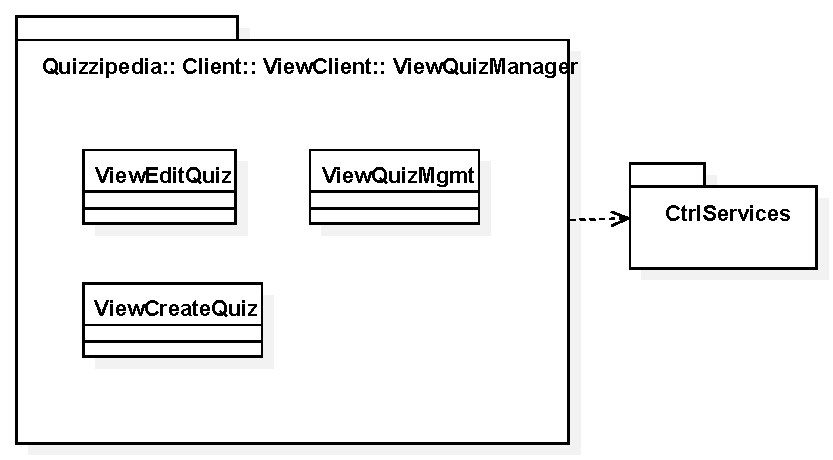
\includegraphics[width=\textwidth]{ImgST/quizzipedia-client-viewclient-viewquizmanager.pdf}}
\caption{Schema Componente Quizzipedia::Client::ViewClient::ViewQuizManager}
\end{figure}
\myparagraph{Classe ViewCreateQuiz}
Presenta la pagina da cui sarà possibile creare un nuovo quiz.
\begin{figure}[H]
\centering
\noindent\makebox[\textwidth]{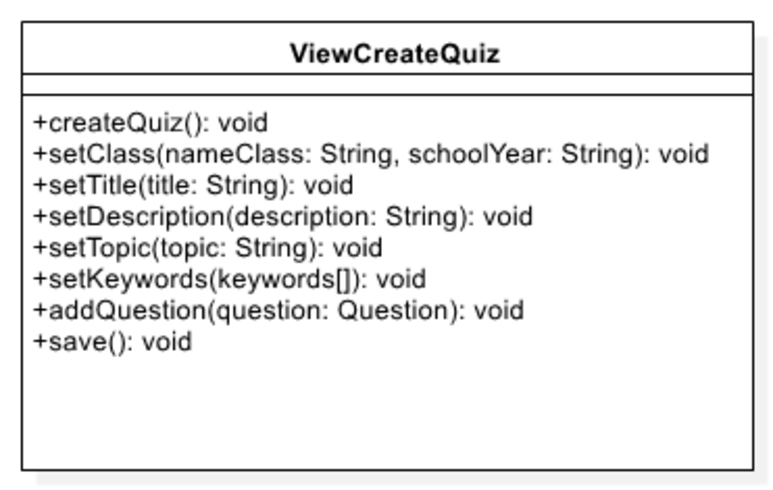
\includegraphics[width=\textwidth]{ImgST/quizzipedia-client-viewclient-viewquizmanager-viewcreatequiz.pdf}}
\caption{Schema Componente Quizzipedia::Client::ViewClient::ViewQuizManager::ViewCreateQuiz}
\end{figure}
\subsubsection{Componente Quizzipedia::Client::ViewClient::ViewQuizSolver}
Il package raccoglie le classi necessarie alla visualizzazione delle pagine da cui sarà possibile svolgere quiz.
\begin{figure}[H]
\centering
\noindent\makebox[\textwidth]{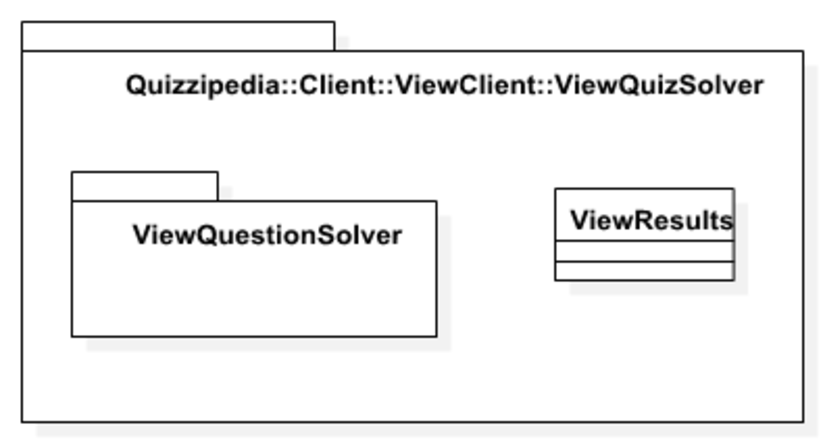
\includegraphics[width=\textwidth]{ImgST/quizzipedia-client-viewclient-viewquizsolver.pdf}}
\caption{Schema Componente Quizzipedia::Client::ViewClient::ViewQuizSolver}
\end{figure}
\myparagraph{Componenti contenute}
\begin{itemize}
\item Quizzipedia::Client::ViewClient::ViewQuizSolver::ViewQuestionSolver
\end{itemize}
\myparagraph{Classe ViewResults}
La classe ha il compito di costruire la pagina da cui sarà possibile vedere l'esito di un quiz.
\begin{figure}[H]
\centering
\noindent\makebox[\textwidth]{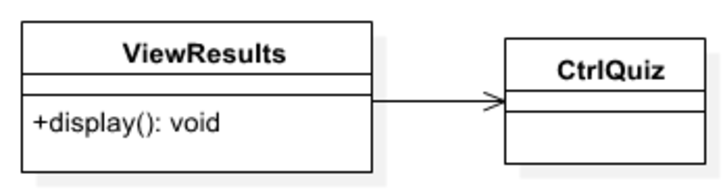
\includegraphics[width=\textwidth]{ImgST/quizzipedia-client-viewclient-viewquizsolver-viewresults.pdf}}
\caption{Schema Componente Quizzipedia::Client::ViewClient::ViewQuizSolver::ViewResults}
\end{figure}
\subsubsection{Componente Quizzipedia::Client::ViewClient::ViewQuizSolver::ViewQuestionSolver}
Il package raccoglie le classi necessarie alla visualizzazione delle pagine da cui sarà possibile rispondere alle singole domande.
\begin{figure}[H]
\centering
\noindent\makebox[\textwidth]{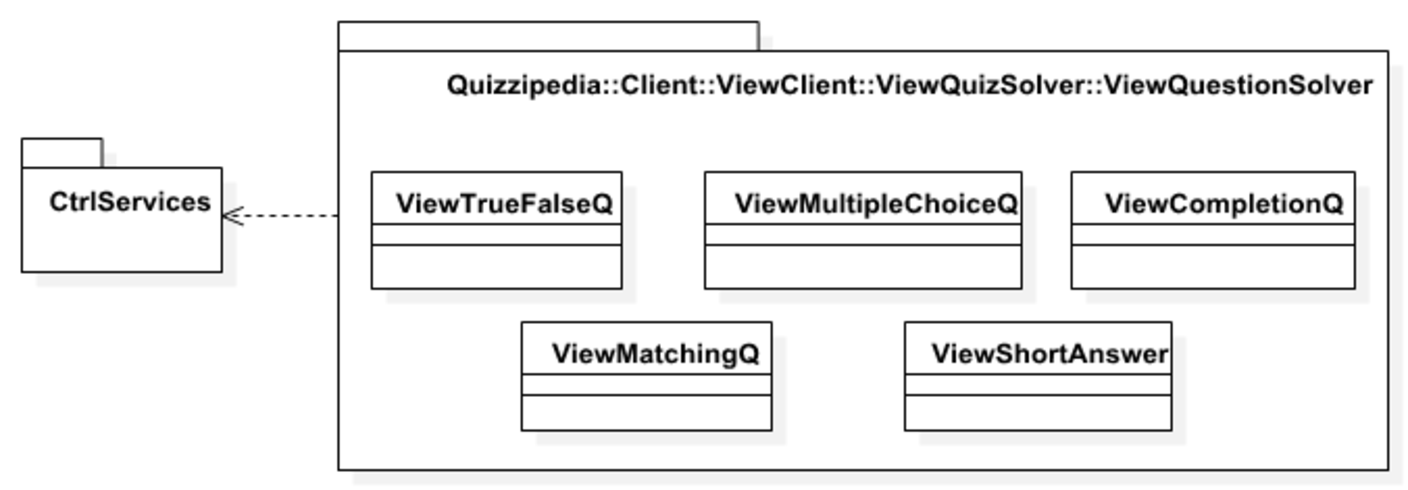
\includegraphics[width=\textwidth]{ImgST/quizzipedia-client-viewclient-viewquizsolver-viewquestionsolver.pdf}}
\caption{Schema Componente Quizzipedia::Client::ViewClient::ViewQuizSolver::ViewQuestionSolver}
\end{figure}
\myparagraph{Classe ViewCompletionQ}
Presenta all'utente la pagina da cui sarà possibile rispondere a una domanda a completamento.
\begin{figure}[H]
\centering
\noindent\makebox[\textwidth]{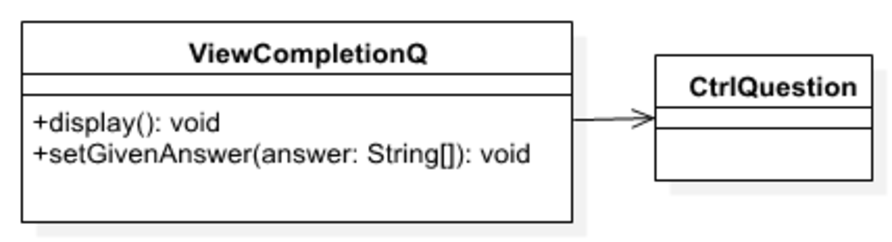
\includegraphics[width=\textwidth]{ImgST/quizzipedia-client-viewclient-viewquizsolver-viewquestionsolver-viewcompletionq.pdf}}
\caption{Schema Componente Quizzipedia::Client::ViewClient::ViewQuizSolver::ViewQuestionSolver::ViewCompletionQ}
\end{figure}
\subsubsection{Componente Quizzipedia::Client::ViewClient::ViewRequests}
Qui sono raccolte le pagine che permettono all'utente di gestire le richieste di ruolo e classe.
\begin{figure}[H]
\centering
\noindent\makebox[\textwidth]{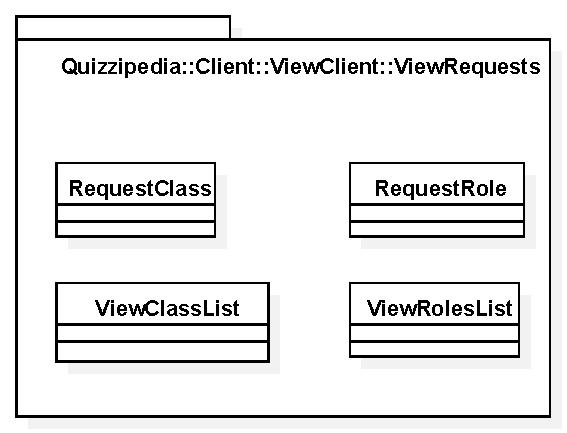
\includegraphics[width=\textwidth]{ImgST/quizzipedia-client-viewclient-viewrequests.pdf}}
\caption{Schema Componente Quizzipedia::Client::ViewClient::ViewRequests}
\end{figure}
\myparagraph{Classe RequestClass}
Costruisce la pagina da cui l'utente potrà richiedere di entrare in una classe.
\begin{figure}[H]
\centering
\noindent\makebox[\textwidth]{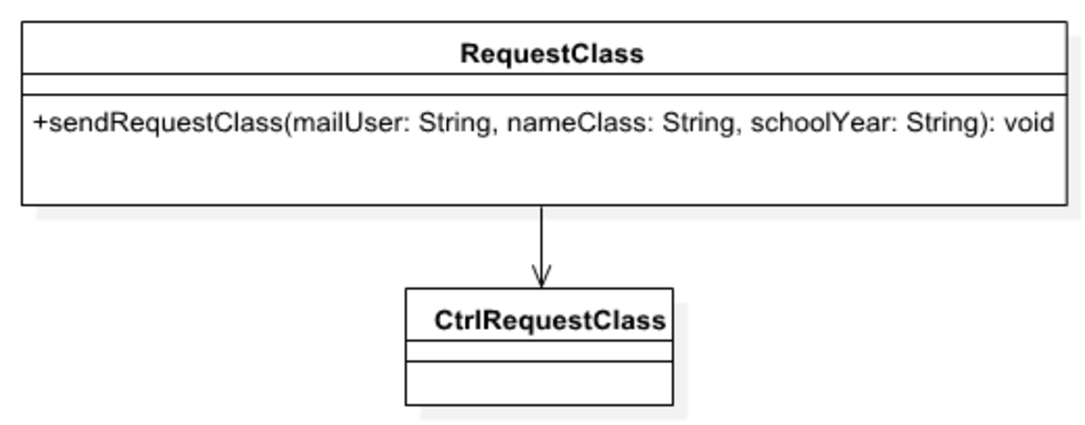
\includegraphics[width=\textwidth]{ImgST/quizzipedia-client-viewclient-viewrequests-requestclass.pdf}}
\caption{Schema Componente Quizzipedia::Client::ViewClient::ViewRequests::RequestClass}
\end{figure}
\subsubsection{Componente Quizzipedia::Client::ViewClient::ViewSearch}
Il package contiene le classi responsabili della creazione delle pagine da cui sarà possibile ricercare domande, quiz e classi .
\begin{figure}[H]
\centering
\noindent\makebox[\textwidth]{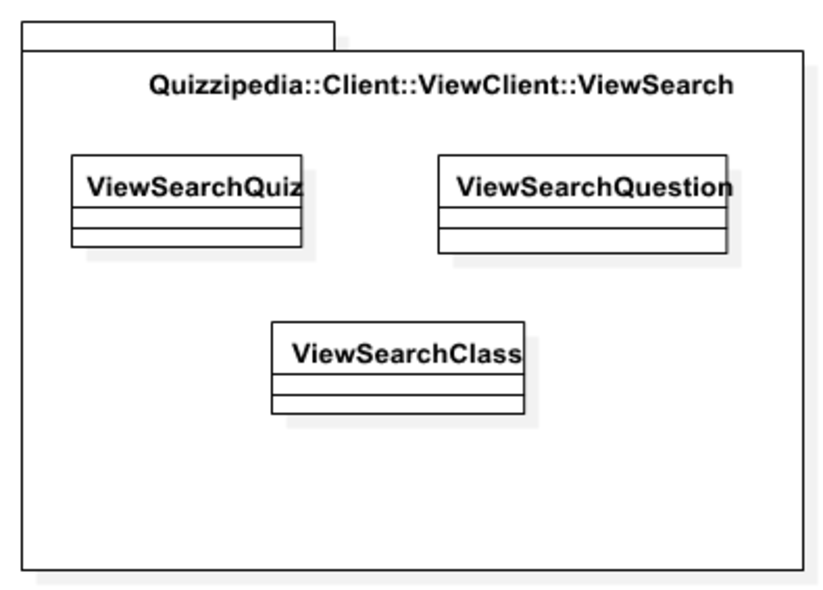
\includegraphics[width=\textwidth]{ImgST/quizzipedia-client-viewclient-viewsearch.pdf}}
\caption{Schema Componente Quizzipedia::Client::ViewClient::ViewSearch}
\end{figure}
\myparagraph{Classe ViewSearchClass}
La classe carica la pagina da cui sarà possibile ricercare classi all'interno di un ente.
\begin{figure}[H]
\centering
\noindent\makebox[\textwidth]{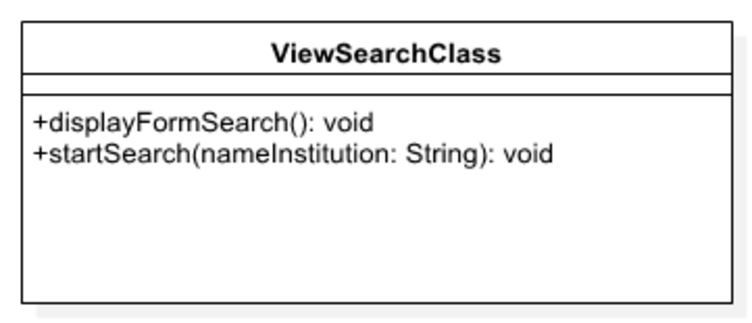
\includegraphics[width=\textwidth]{ImgST/quizzipedia-client-viewclient-viewsearch-viewsearchclass.pdf}}
\caption{Schema Componente Quizzipedia::Client::ViewClient::ViewSearch::ViewSearchClass}
\end{figure}
\subsubsection{Componente Quizzipedia::Client::ViewClient::ViewStatistics}
Package che gestisce le pagine in cui verranno visualizzate le statistiche.
\begin{figure}[H]
\centering
\noindent\makebox[\textwidth]{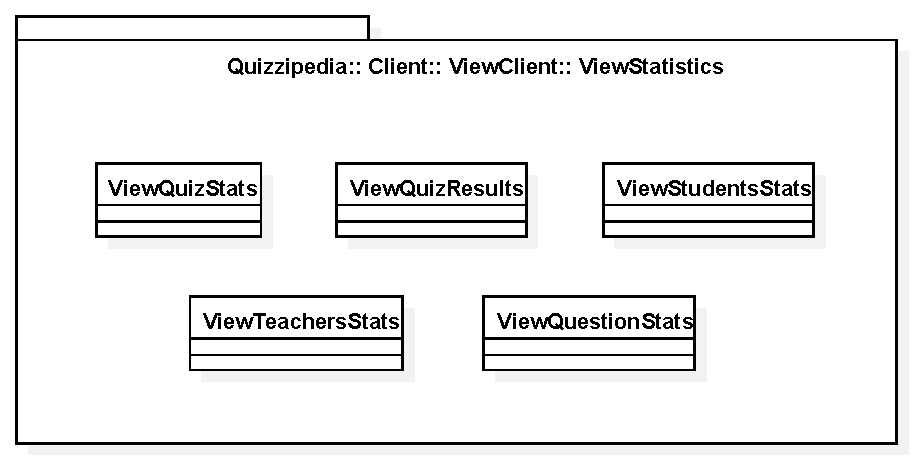
\includegraphics[width=\textwidth]{ImgST/quizzipedia-client-viewclient-viewstatistics.pdf}}
\caption{Schema Componente Quizzipedia::Client::ViewClient::ViewStatistics}
\end{figure}
\myparagraph{Classe VieewQuizStats}
Vengono rappresentate le statistiche generali riguardanti i quiz.
\begin{figure}[H]
\centering
\noindent\makebox[\textwidth]{\includegraphics[width=\textwidth]{ImgST/quizzipedia-client-viewclient-viewstatistics-vieewquizstats.pdf}}
\caption{Schema Componente Quizzipedia::Client::ViewClient::ViewStatistics::VieewQuizStats}
\end{figure}
\subsubsection{Componente Quizzipedia::Client::ViewClient::ViewTopicManager}
Qui sono raccolte le classi responsabili della presentazione delle pagine da cui sarà possibile gestire gli argomenti di domande e quiz.
\begin{figure}[H]
\centering
\noindent\makebox[\textwidth]{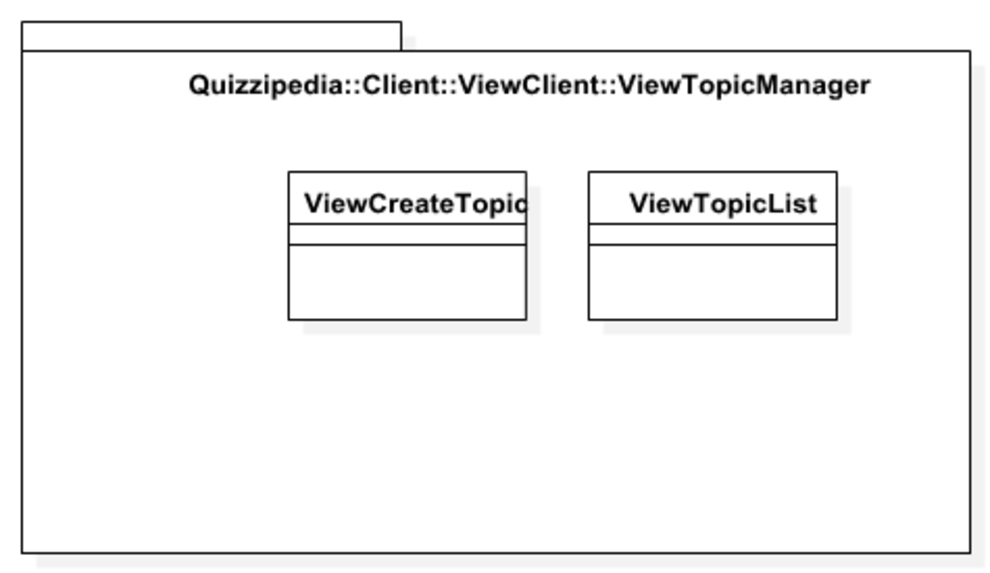
\includegraphics[width=\textwidth]{ImgST/quizzipedia-client-viewclient-viewtopicmanager.pdf}}
\caption{Schema Componente Quizzipedia::Client::ViewClient::ViewTopicManager}
\end{figure}
\myparagraph{Classe ViewCreateTopic}
La classe caricherà la pagina da cui sarà possibile creare un nuovo argomento.
\begin{figure}[H]
\centering
\noindent\makebox[\textwidth]{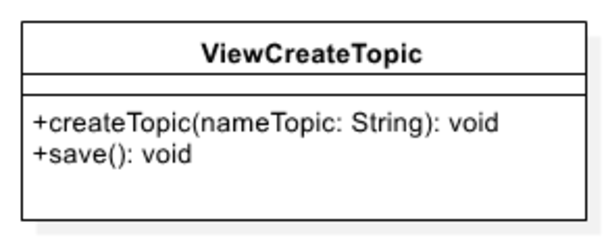
\includegraphics[width=\textwidth]{ImgST/quizzipedia-client-viewclient-viewtopicmanager-viewcreatetopic.pdf}}
\caption{Schema Componente Quizzipedia::Client::ViewClient::ViewTopicManager::ViewCreateTopic}
\end{figure}
\subsubsection{Componente Quizzipedia::Client::ViewClient::ViewUsers}
Raccoglie le classi necessarie a presentare all'utente le pagine da cui visualizzare le informazioni che lo riguardano e compiere le funzioni principali.
\begin{figure}[H]
\centering
\noindent\makebox[\textwidth]{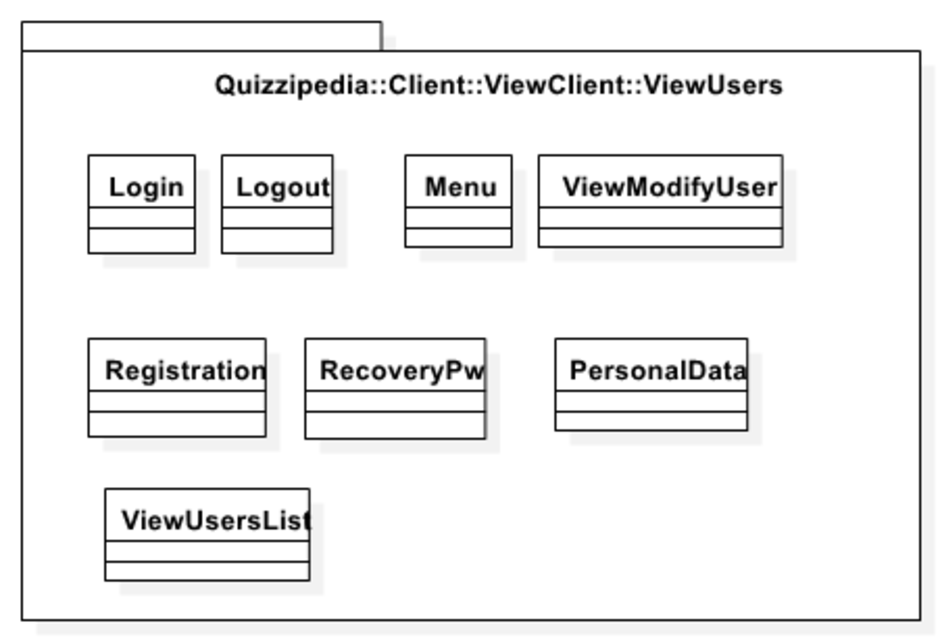
\includegraphics[width=\textwidth]{ImgST/quizzipedia-client-viewclient-viewusers.pdf}}
\caption{Schema Componente Quizzipedia::Client::ViewClient::ViewUsers}
\end{figure}
\myparagraph{Classe Login}
Presenta la pagina necessaria per effettuare il login nel sistema.
\begin{figure}[H]
\centering
\noindent\makebox[\textwidth]{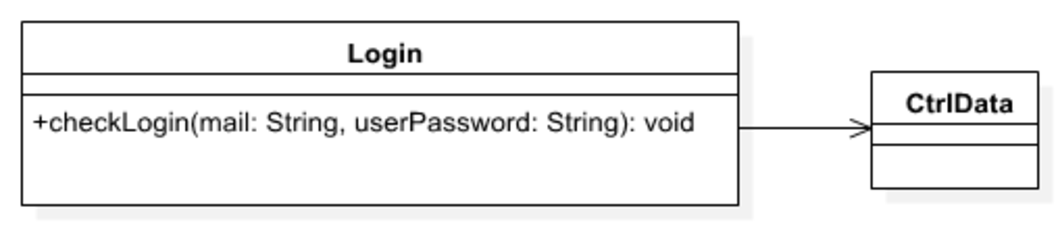
\includegraphics[width=\textwidth]{ImgST/quizzipedia-client-viewclient-viewusers-login.pdf}}
\caption{Schema Componente Quizzipedia::Client::ViewClient::ViewUsers::Login}
\end{figure}
\subsubsection{Componente Quizzipedia::Client::ControllerClient}
Raccoglie le classi responsabili della comunicazione tra il model e la view.
\begin{figure}[H]
\centering
\noindent\makebox[\textwidth]{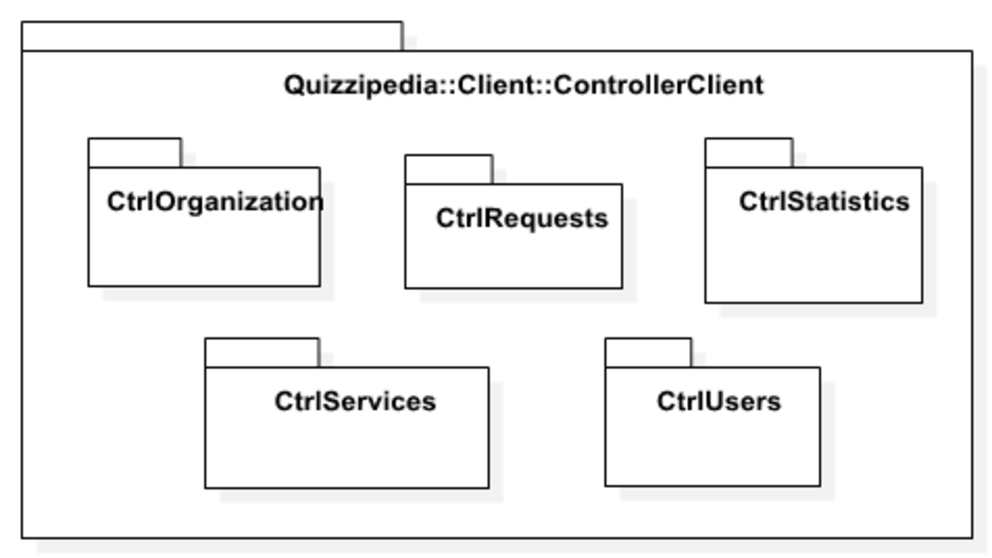
\includegraphics[width=\textwidth]{ImgST/quizzipedia-client-controllerclient.pdf}}
\caption{Schema Componente Quizzipedia::Client::ControllerClient}
\end{figure}
\myparagraph{Componenti contenute}
\begin{itemize}
\item Quizzipedia::Client::ControllerClient::CtrlOrganization
\item Quizzipedia::Client::ControllerClient::CtrlRequests
\item Quizzipedia::Client::ControllerClient::CtrlServices
\item Quizzipedia::Client::ControllerClient::CtrlStatistics
\item Quizzipedia::Client::ControllerClient::CtrlUsers
\end{itemize}
\subsubsection{Componente Quizzipedia::Client::ControllerClient::CtrlOrganization}
Raccoglie le classi che si occupano delle comunicazioni necessarie per la creazione di enti e classi.
\begin{figure}[H]
\centering
\noindent\makebox[\textwidth]{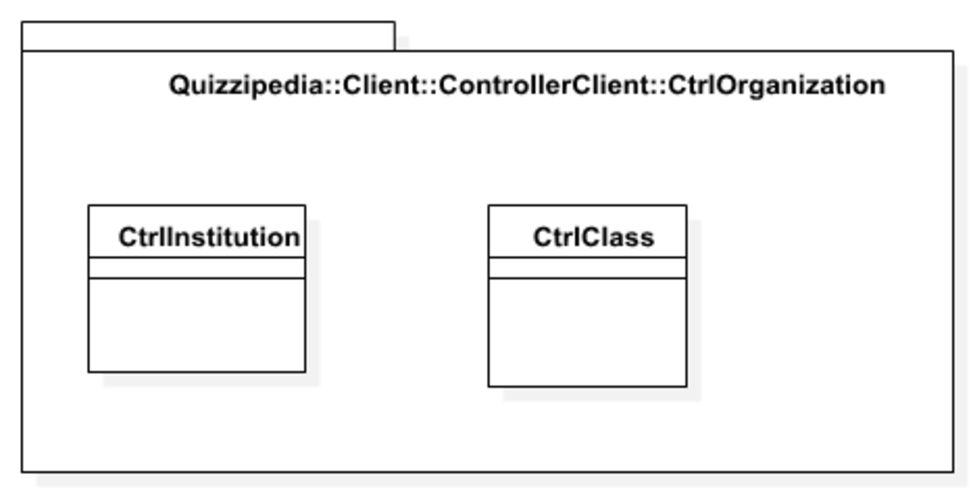
\includegraphics[width=\textwidth]{ImgST/quizzipedia-client-controllerclient-ctrlorganization.pdf}}
\caption{Schema Componente Quizzipedia::Client::ControllerClient::CtrlOrganization}
\end{figure}
\myparagraph{Classe CtrlClass}
Vi sono presenti metodi necessari alla creazione delle classi.
\begin{figure}[H]
\centering
\noindent\makebox[\textwidth]{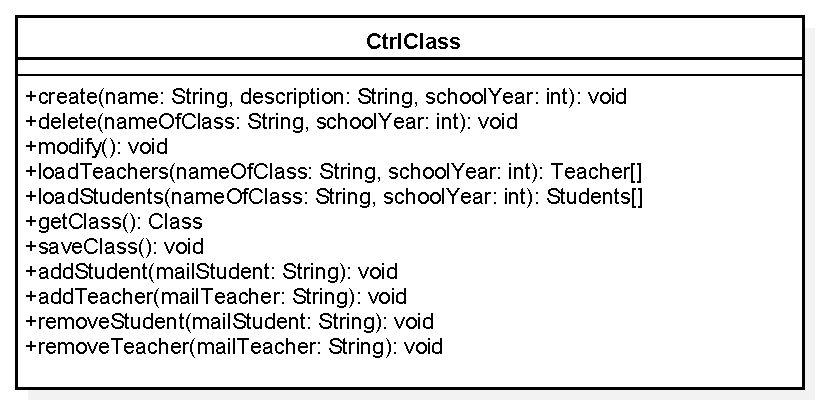
\includegraphics[width=\textwidth]{ImgST/quizzipedia-client-controllerclient-ctrlorganization-ctrlclass.pdf}}
\caption{Schema Componente Quizzipedia::Client::ControllerClient::CtrlOrganization::CtrlClass}
\end{figure}
\subsubsection{Componente Quizzipedia::Client::ControllerClient::CtrlRequests}
Questo package contiene classi necessarie alla gestione delle richieste di ruolo o classe.
\begin{figure}[H]
\centering
\noindent\makebox[\textwidth]{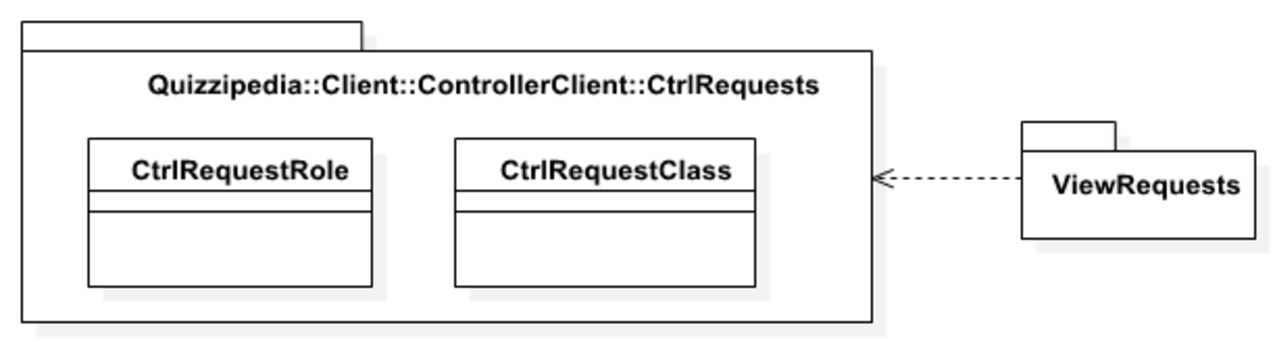
\includegraphics[width=\textwidth]{ImgST/quizzipedia-client-controllerclient-ctrlrequests.pdf}}
\caption{Schema Componente Quizzipedia::Client::ControllerClient::CtrlRequests}
\end{figure}
\myparagraph{Classe CtrlRequestClass}
Si occupa delle comunicazioni necessarie per la gestione delle richieste di inserimento in una classe.
\begin{figure}[H]
\centering
\noindent\makebox[\textwidth]{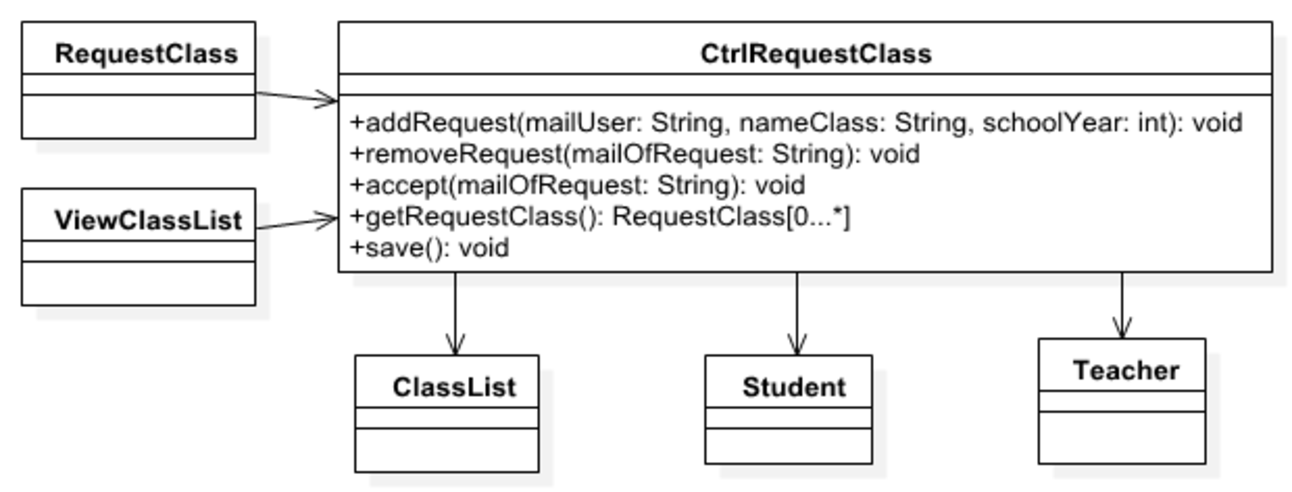
\includegraphics[width=\textwidth]{ImgST/quizzipedia-client-controllerclient-ctrlrequests-ctrlrequestclass.pdf}}
\caption{Schema Componente Quizzipedia::Client::ControllerClient::CtrlRequests::CtrlRequestClass}
\end{figure}
\subsubsection{Componente Quizzipedia::Client::ControllerClient::CtrlServices}
Raccoglie gli elementi necessari alla creazione, svolgimento e ricerca di quiz e domande.
\begin{figure}[H]
\centering
\noindent\makebox[\textwidth]{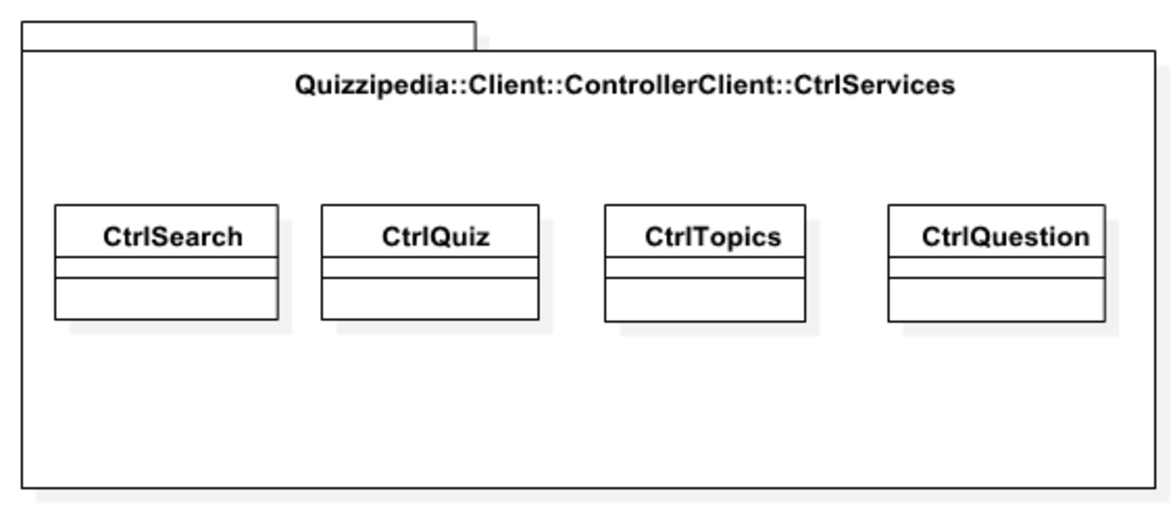
\includegraphics[width=\textwidth]{ImgST/quizzipedia-client-controllerclient-ctrlservices.pdf}}
\caption{Schema Componente Quizzipedia::Client::ControllerClient::CtrlServices}
\end{figure}
\myparagraph{Classe CtrlQuestion}
Fornisce i metodi necessari per la comunicazione tra view e model durante la creazione, modifica e svolgimento di una domanda.
\begin{figure}[H]
\centering
\noindent\makebox[\textwidth]{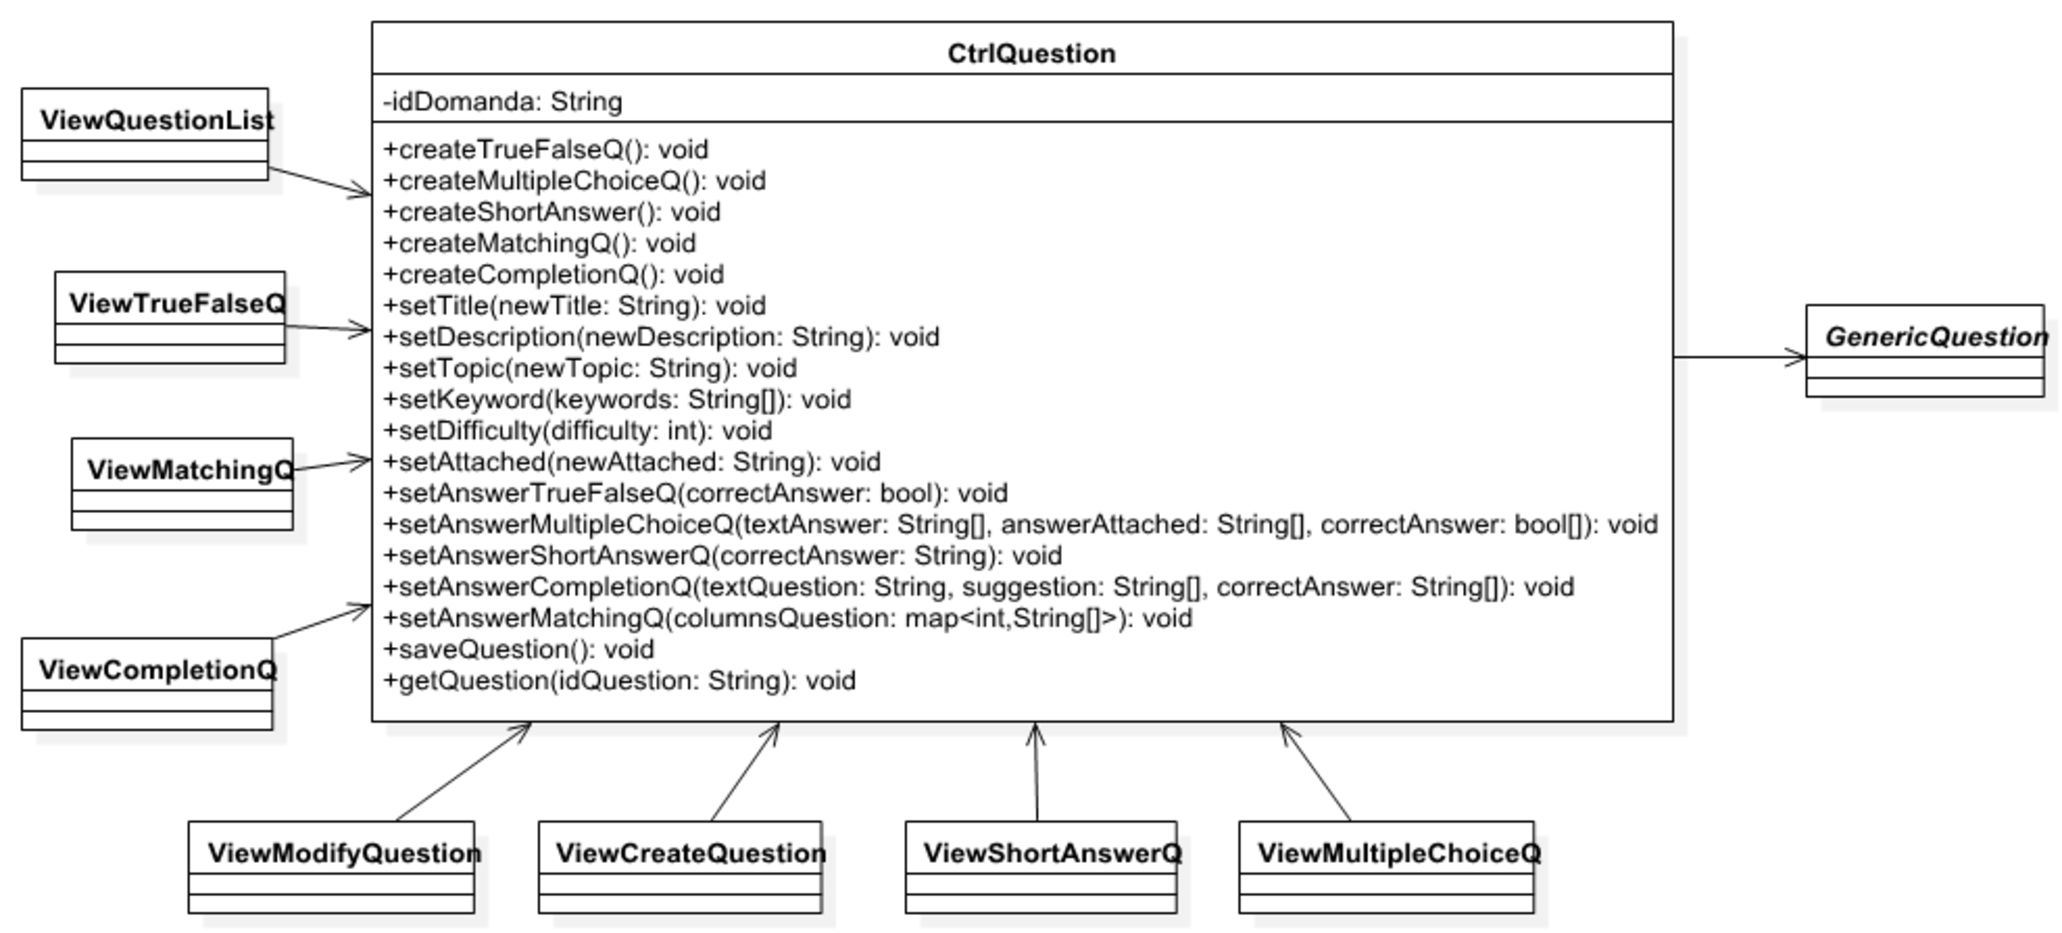
\includegraphics[width=\textwidth]{ImgST/quizzipedia-client-controllerclient-ctrlservices-ctrlquestion.pdf}}
\caption{Schema Componente Quizzipedia::Client::ControllerClient::CtrlServices::CtrlQuestion}
\end{figure}
\subsubsection{Componente Quizzipedia::Client::ControllerClient::CtrlStatistics}
Raccoglie le classi necessarie a recuperare le statistiche da presentare all'utente.
\begin{figure}[H]
\centering
\noindent\makebox[\textwidth]{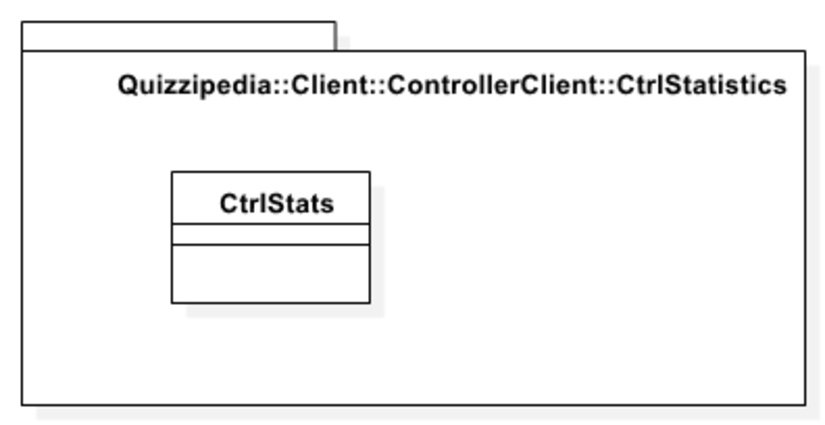
\includegraphics[width=\textwidth]{ImgST/quizzipedia-client-controllerclient-ctrlstatistics.pdf}}
\caption{Schema Componente Quizzipedia::Client::ControllerClient::CtrlStatistics}
\end{figure}
\myparagraph{Classe CtrlStats}
Classe necessaria al caricamento delle statistiche relative ai quiz, alle domande e alle classi.
\begin{figure}[H]
\centering
\noindent\makebox[\textwidth]{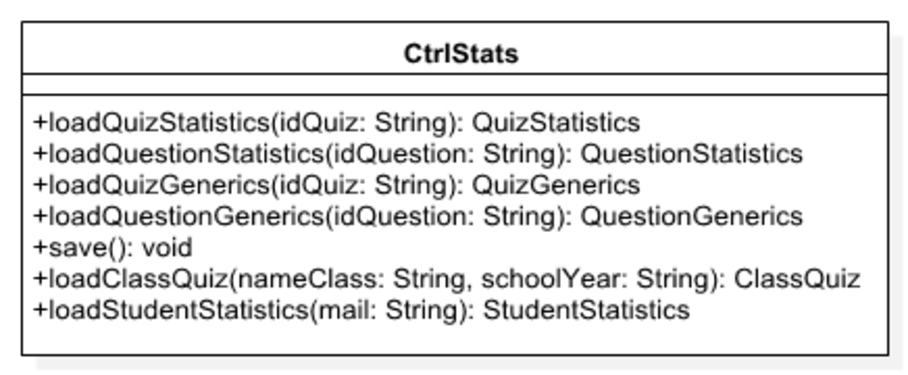
\includegraphics[width=\textwidth]{ImgST/quizzipedia-client-controllerclient-ctrlstatistics-ctrlstats.pdf}}
\caption{Schema Componente Quizzipedia::Client::ControllerClient::CtrlStatistics::CtrlStats}
\end{figure}
\subsubsection{Componente Quizzipedia::Client::ControllerClient::CtrlUsers}
Il package raccoglie le classi che permettono la comunicazione per quanto riguarda funzioni e dati dell'utente.
\begin{figure}[H]
\centering
\noindent\makebox[\textwidth]{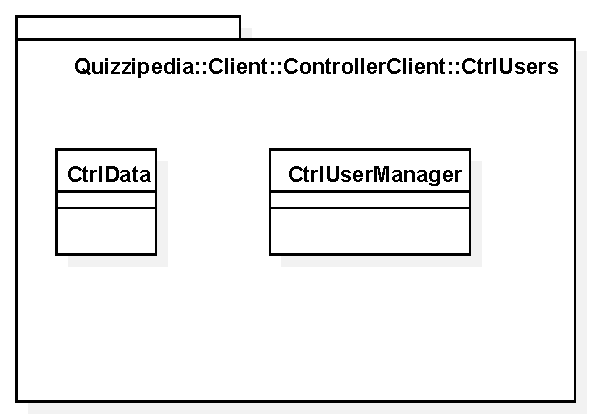
\includegraphics[width=\textwidth]{ImgST/quizzipedia-client-controllerclient-ctrlusers.pdf}}
\caption{Schema Componente Quizzipedia::Client::ControllerClient::CtrlUsers}
\end{figure}
\myparagraph{Classe CtrlData}
La classe raccoglie i metodi per gestire le informazioni personali di tutti gli utenti autenticati.
\begin{figure}[H]
\centering
\noindent\makebox[\textwidth]{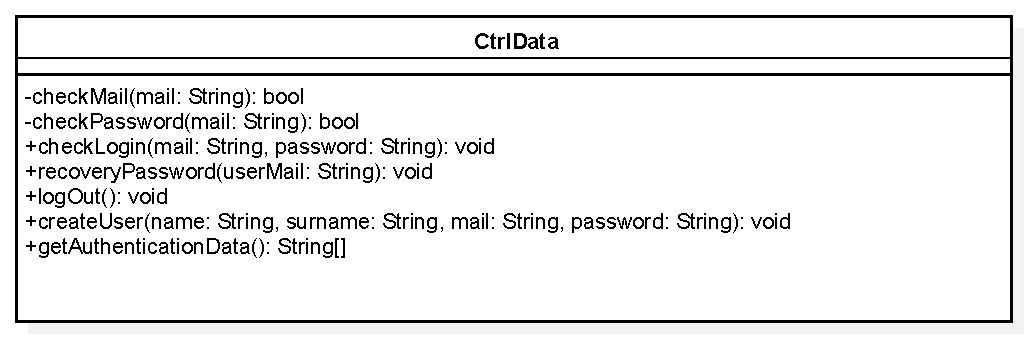
\includegraphics[width=\textwidth]{ImgST/quizzipedia-client-controllerclient-ctrlusers-ctrldata.pdf}}
\caption{Schema Componente Quizzipedia::Client::ControllerClient::CtrlUsers::CtrlData}
\end{figure}
\subsection{Server}
Racchiude tutte le componenti necessarie per il back-end del prodotto. Contiene anche le componenti che si occupano del QML.
\begin{figure}[H]
\centering
\noindent\makebox[\textwidth]{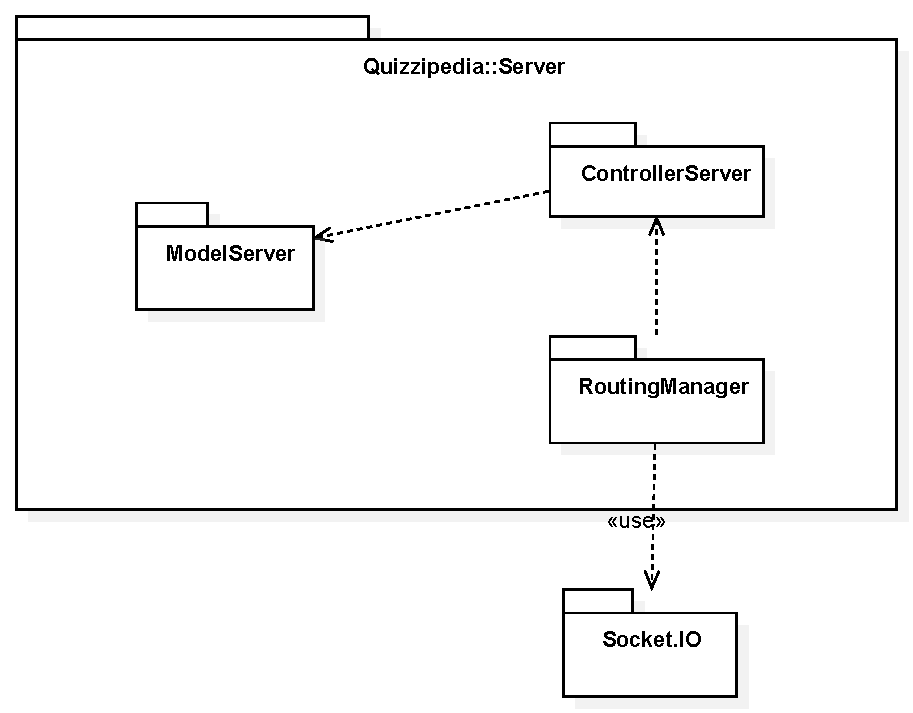
\includegraphics[width=\textwidth]{ImgST/quizzipedia-server.pdf}}
\caption{Schema Componente Quizzipedia::Server}
\end{figure}
\subsubsection{Componente Quizzipedia::Server::ModelServer}
Rappresenta il modello dei dati che verranno utilizzati dal sistema lato server.
\begin{figure}[H]
\centering
\noindent\makebox[\textwidth]{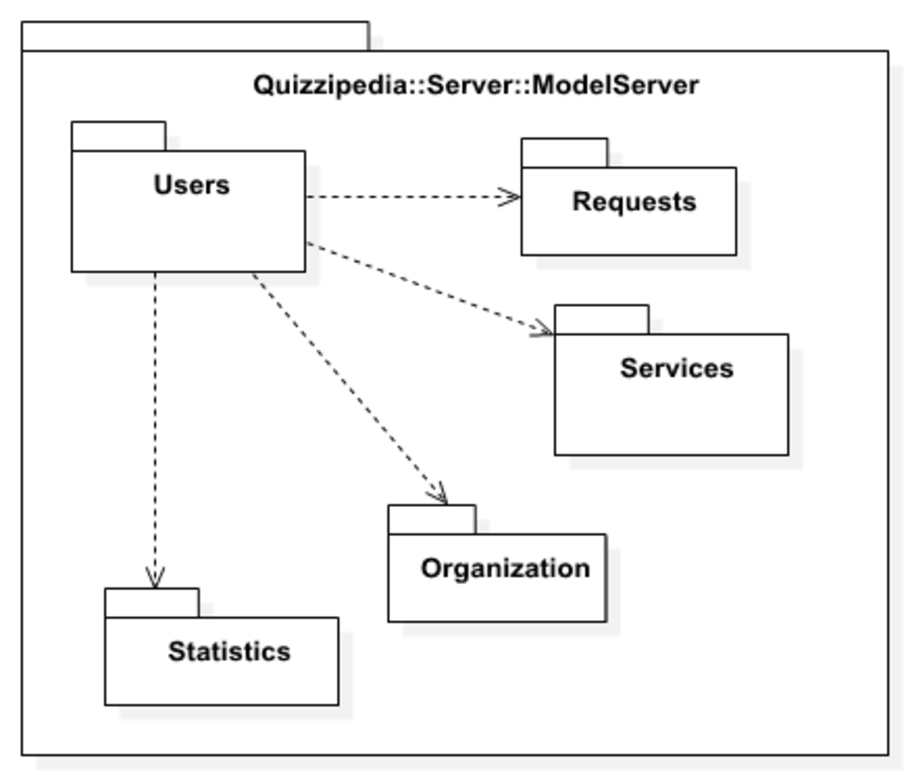
\includegraphics[width=\textwidth]{ImgST/quizzipedia-server-modelserver.pdf}}
\caption{Schema Componente Quizzipedia::Server::ModelServer}
\end{figure}
\myparagraph{Componenti contenute}
\begin{itemize}
\item Quizzipedia::Server::ModelServer::Services1
\end{itemize}
\subsubsection{Componente Quizzipedia::Server::ModelServer::Services1}
Il package racchiude i modelli necessari alla creazione di domande e quiz, i servizi principali offerti dal nostro prodotto.
\begin{figure}[H]
\centering
\noindent\makebox[\textwidth]{\includegraphics[width=\textwidth]{ImgST/quizzipedia-server-modelserver-services1.pdf}}
\caption{Schema Componente Quizzipedia::Server::ModelServer::Services1}
\end{figure}
\myparagraph{Componenti contenute}
\begin{itemize}
\item Quizzipedia::Server::ModelServer::Services1::Questions1
\end{itemize}
\myparagraph{Classe Info1}
Riassume le informazioni principali su quiz e domande, necessarie per una presentazione sintetica e puntuale all'utente. È poi possibile risalire alla domanda o al quiz completi.
\begin{figure}[H]
\centering
\noindent\makebox[\textwidth]{\includegraphics[width=\textwidth]{ImgST/quizzipedia-server-modelserver-services1-info1.pdf}}
\caption{Schema Componente Quizzipedia::Server::ModelServer::Services1::Info1}
\end{figure}
\subsubsection{Componente Quizzipedia::Server::ModelServer::Services1::Questions1}
Descrive il modo in cui sono strutturati i vari tipi di domande che l'utente può incontrare durante la creazione o la compilazione di quiz.
\begin{figure}[H]
\centering
\noindent\makebox[\textwidth]{\includegraphics[width=\textwidth]{ImgST/quizzipedia-server-modelserver-services1-questions1.pdf}}
\caption{Schema Componente Quizzipedia::Server::ModelServer::Services1::Questions1}
\end{figure}
\myparagraph{Classe Cell1}
La classe descrive ogni singola riga (quindi ogni opzione) della colonna della domanda a collegamento.
\begin{figure}[H]
\centering
\noindent\makebox[\textwidth]{\includegraphics[width=\textwidth]{ImgST/quizzipedia-server-modelserver-services1-questions1-cell1.pdf}}
\caption{Schema Componente Quizzipedia::Server::ModelServer::Services1::Questions1::Cell1}
\end{figure}
\subsubsection{Componente Quizzipedia::Server::ControllerServer}
Questo package contiene tutti i servizi che ricalcano il pattern architetturale DAO in modo da isolare l'accesso al database relazionale, controllando sempre che l'utente che genera una determinata richiesta al server sia abilitato per farla.
\begin{figure}[H]
\centering
\noindent\makebox[\textwidth]{\includegraphics[width=\textwidth]{ImgST/quizzipedia-server-controllerserver.pdf}}
\caption{Schema Componente Quizzipedia::Server::ControllerServer}
\end{figure}
\myparagraph{Componenti contenute}
\begin{itemize}
\item Quizzipedia::Server::ControllerServer::AuthenticationManager
\item Quizzipedia::Server::ControllerServer::ClassManager
\item Quizzipedia::Server::ControllerServer::ProfileManager
\item Quizzipedia::Server::ControllerServer::QuizManager
\item Quizzipedia::Server::ControllerServer::RequestsManager
\item Quizzipedia::Server::ControllerServer::SearchManager
\item Quizzipedia::Server::ControllerServer::StatisticsManager
\item Quizzipedia::Server::ControllerServer::TopicManager
\end{itemize}
\subsubsection{Componente Quizzipedia::Server::ControllerServer::AuthenticationManager}
Package che permette di gestire le funzioni basi per una corretta autenticazione al sistema.
\begin{figure}[H]
\centering
\noindent\makebox[\textwidth]{\includegraphics[width=\textwidth]{ImgST/quizzipedia-server-controllerserver-authenticationmanager.pdf}}
\caption{Schema Componente Quizzipedia::Server::ControllerServer::AuthenticationManager}
\end{figure}
\myparagraph{Classe LoggerIn}
Permette l'autenticazione nel sistema da parte di utenti preventivamente registrati.
\begin{figure}[H]
\centering
\noindent\makebox[\textwidth]{\includegraphics[width=\textwidth]{ImgST/quizzipedia-server-controllerserver-authenticationmanager-loggerin.pdf}}
\caption{Schema Componente Quizzipedia::Server::ControllerServer::AuthenticationManager::LoggerIn}
\end{figure}
\subsubsection{Componente Quizzipedia::Server::ControllerServer::ClassManager}
Package che racchiude tutte le funzionalità adibite al salvataggio e alla visualizzazione delle informazioni riguardanti le classi di un ente.
\begin{figure}[H]
\centering
\noindent\makebox[\textwidth]{\includegraphics[width=\textwidth]{ImgST/quizzipedia-server-controllerserver-classmanager.pdf}}
\caption{Schema Componente Quizzipedia::Server::ControllerServer::ClassManager}
\end{figure}
\myparagraph{Classe AddClass}
Permette la creazione di una nuova classe.
\begin{figure}[H]
\centering
\noindent\makebox[\textwidth]{\includegraphics[width=\textwidth]{ImgST/quizzipedia-server-controllerserver-classmanager-addclass.pdf}}
\caption{Schema Componente Quizzipedia::Server::ControllerServer::ClassManager::AddClass}
\end{figure}
\subsubsection{Componente Quizzipedia::Server::ControllerServer::ProfileManager}
Package che racchiude tutte le funzionalità adibite al salvataggio e alla visualizzazione delle informazioni personali da parte di un utente autenticato.
\begin{figure}[H]
\centering
\noindent\makebox[\textwidth]{\includegraphics[width=\textwidth]{ImgST/quizzipedia-server-controllerserver-profilemanager.pdf}}
\caption{Schema Componente Quizzipedia::Server::ControllerServer::ProfileManager}
\end{figure}
\myparagraph{Classe AccountDeleter}
Permette la rimozione di un account dal sistema.
\begin{figure}[H]
\centering
\noindent\makebox[\textwidth]{\includegraphics[width=\textwidth]{ImgST/quizzipedia-server-controllerserver-profilemanager-accountdeleter.pdf}}
\caption{Schema Componente Quizzipedia::Server::ControllerServer::ProfileManager::AccountDeleter}
\end{figure}
\subsubsection{Componente Quizzipedia::Server::ControllerServer::QuizManager}
Package che racchiude tutte le funzionalità adibite alla creazione, modifica e al recupero di quiz per lo svolgimento da parte di un utente.
\begin{figure}[H]
\centering
\noindent\makebox[\textwidth]{\includegraphics[width=\textwidth]{ImgST/quizzipedia-server-controllerserver-quizmanager.pdf}}
\caption{Schema Componente Quizzipedia::Server::ControllerServer::QuizManager}
\end{figure}
\myparagraph{Componenti contenute}
\begin{itemize}
\item Quizzipedia::Server::ControllerServer::QuizManager::QMLAgent
\end{itemize}
\myparagraph{Classe QuizCreator}
Permette il salvataggio nella base di dati di un nuovo quiz.
\begin{figure}[H]
\centering
\noindent\makebox[\textwidth]{\includegraphics[width=\textwidth]{ImgST/quizzipedia-server-controllerserver-quizmanager-quizcreator.pdf}}
\caption{Schema Componente Quizzipedia::Server::ControllerServer::QuizManager::QuizCreator}
\end{figure}
\subsubsection{Componente Quizzipedia::Server::ControllerServer::QuizManager::QMLAgent}
Questo package racchiude i moduli necessari alla traduzione da QML ad un formato comprensibile dal sistema le informazioni estratte dal database per la generazione delle pagine HTML relative ad un quiz e viceversa.
\begin{figure}[H]
\centering
\noindent\makebox[\textwidth]{\includegraphics[width=\textwidth]{ImgST/quizzipedia-server-controllerserver-quizmanager-qmlagent.pdf}}
\caption{Schema Componente Quizzipedia::Server::ControllerServer::QuizManager::QMLAgent}
\end{figure}
\myparagraph{Classe QMLGenerator}
Permette la traduzione in formato QML di un quiz nel caso si voglia procedere al salvataggio dello stesso all'interno del database.
\begin{figure}[H]
\centering
\noindent\makebox[\textwidth]{\includegraphics[width=\textwidth]{ImgST/quizzipedia-server-controllerserver-quizmanager-qmlagent-qmlgenerator.pdf}}
\caption{Schema Componente Quizzipedia::Server::ControllerServer::QuizManager::QMLAgent::QMLGenerator}
\end{figure}
\subsubsection{Componente Quizzipedia::Server::ControllerServer::RequestsManager}
Package che si occupa di memorizzare richieste da parte degli utenti, mostrarle al responsabile e permettergli di accettarle o meno.
\begin{figure}[H]
\centering
\noindent\makebox[\textwidth]{\includegraphics[width=\textwidth]{ImgST/quizzipedia-server-controllerserver-requestsmanager.pdf}}
\caption{Schema Componente Quizzipedia::Server::ControllerServer::RequestsManager}
\end{figure}
\myparagraph{Classe ClassRequestsAdder}
Permette la memorizzazione delle richieste di creazione di una classe.
\begin{figure}[H]
\centering
\noindent\makebox[\textwidth]{\includegraphics[width=\textwidth]{ImgST/quizzipedia-server-controllerserver-requestsmanager-classrequestsadder.pdf}}
\caption{Schema Componente Quizzipedia::Server::ControllerServer::RequestsManager::ClassRequestsAdder}
\end{figure}
\subsubsection{Componente Quizzipedia::Server::ControllerServer::SearchManager}
Questo package permette di effettuare una ricerca nel database di quiz o domande richiesti dall'utente e ritornare una lista che corrisponde ai parametri desiderati.
\begin{figure}[H]
\centering
\noindent\makebox[\textwidth]{\includegraphics[width=\textwidth]{ImgST/quizzipedia-server-controllerserver-searchmanager.pdf}}
\caption{Schema Componente Quizzipedia::Server::ControllerServer::SearchManager}
\end{figure}
\myparagraph{Classe QuestionSearcher}
Ritorna una lista di domande che corrispondono ai parametri di ricerca impostati dall'utente.
\begin{figure}[H]
\centering
\noindent\makebox[\textwidth]{\includegraphics[width=\textwidth]{ImgST/quizzipedia-server-controllerserver-searchmanager-questionsearcher.pdf}}
\caption{Schema Componente Quizzipedia::Server::ControllerServer::SearchManager::QuestionSearcher}
\end{figure}
\subsubsection{Componente Quizzipedia::Server::ControllerServer::StatisticsManager}
Questo package ha il compito di recuperare tutte le informazioni sottoforma di statistiche relative ad un quiz, una domanda in particolare o ad un utente.
\begin{figure}[H]
\centering
\noindent\makebox[\textwidth]{\includegraphics[width=\textwidth]{ImgST/quizzipedia-server-controllerserver-statisticsmanager.pdf}}
\caption{Schema Componente Quizzipedia::Server::ControllerServer::StatisticsManager}
\end{figure}
\myparagraph{Classe PersonalStatisticsFetcher}
Ritorna le statistiche personali.
\begin{figure}[H]
\centering
\noindent\makebox[\textwidth]{\includegraphics[width=\textwidth]{ImgST/quizzipedia-server-controllerserver-statisticsmanager-personalstatisticsfetcher.pdf}}
\caption{Schema Componente Quizzipedia::Server::ControllerServer::StatisticsManager::PersonalStatisticsFetcher}
\end{figure}
\subsubsection{Componente Quizzipedia::Server::ControllerServer::TopicManager}
Package che permette la creazione di un nuovo argomento o l'eliminazione di uno già esistente.
\begin{figure}[H]
\centering
\noindent\makebox[\textwidth]{\includegraphics[width=\textwidth]{ImgST/quizzipedia-server-controllerserver-topicmanager.pdf}}
\caption{Schema Componente Quizzipedia::Server::ControllerServer::TopicManager}
\end{figure}
\myparagraph{Classe SessionController8}
Effettua il controllo sull'utente per verificare che egli sia in possesso dell'autorizzazione necessaria per compiere determinate richieste alla base di dati.
\begin{figure}[H]
\centering
\noindent\makebox[\textwidth]{\includegraphics[width=\textwidth]{ImgST/quizzipedia-server-controllerserver-topicmanager-sessioncontroller8.pdf}}
\caption{Schema Componente Quizzipedia::Server::ControllerServer::TopicManager::SessionController8}
\end{figure}
\subsubsection{Componente Quizzipedia::Server::RoutingManager}
Questo pachetto costituisce lo strato superiore a ControllerServer e contiene tutte le API necessarie per comunicare con il client tramite socket; esso ha il compito di indirizzare le richieste ai vari services un base alla richiesta da parte dell'utente.
\begin{figure}[H]
\centering
\noindent\makebox[\textwidth]{\includegraphics[width=\textwidth]{ImgST/quizzipedia-server-routingmanager.pdf}}
\caption{Schema Componente Quizzipedia::Server::RoutingManager}
\end{figure}
\myparagraph{Classe AuthenticationRouter}
Invocato dal client per interagire con AuthenticationManager.
\begin{figure}[H]
\centering
\noindent\makebox[\textwidth]{\includegraphics[width=\textwidth]{ImgST/quizzipedia-server-routingmanager-authenticationrouter.pdf}}
\caption{Schema Componente Quizzipedia::Server::RoutingManager::AuthenticationRouter}
\end{figure}
